\documentclass[russian, hyperref={unicode}]{beamer}

\usetheme{Madrid}
\setbeamertemplate{footline}[frame number]
\setbeamertemplate{navigation symbols}{}

\usepackage[T2A]{fontenc}
\usepackage{lmodern}
\usepackage[utf8x]{inputenc}
\usepackage[english, russian]{babel}
\usepackage{graphicx}

\theoremstyle{definition}
\newtheorem{rudefinition}{Определение}

\graphicspath{ {../Images/} }

% workaroung warning
\let\Tiny=\tiny

\title{Построение семейств оптимальных маршрутов на морских картах}
\author{Иван Громаковский \\
Научный руководитель: А. С. Ковалев}
\institute{Санкт-Петербургский национальный исследовательский университет \\ информационных технологий, механики и оптики}
\date{}

\begin{document}

\section{Введение}

\frame{\titlepage}
\note{Здравствуйте!}

\subsection{Неформальная постановка}

\begin{frame}{Описание задачи}
    \only<1-3> {
        \begin{itemize}
            \item Имеется морская навигационная карта
            \item Требуется предоставить возможность найти как можно
              больше непохожих маршрутов между двумя точками
            \item Задача поддержки принятия решения ⇒ real time
            \item<2-3> \alert{Не требуется находить кратчайший маршрут, однако
              маршруты должны быть не сильно длиннее кратчайшего}
        \end{itemize}
        \uncover<3> {
            \begin{columns}
                \column{.5\textwidth}
                    \begin{figure}
                        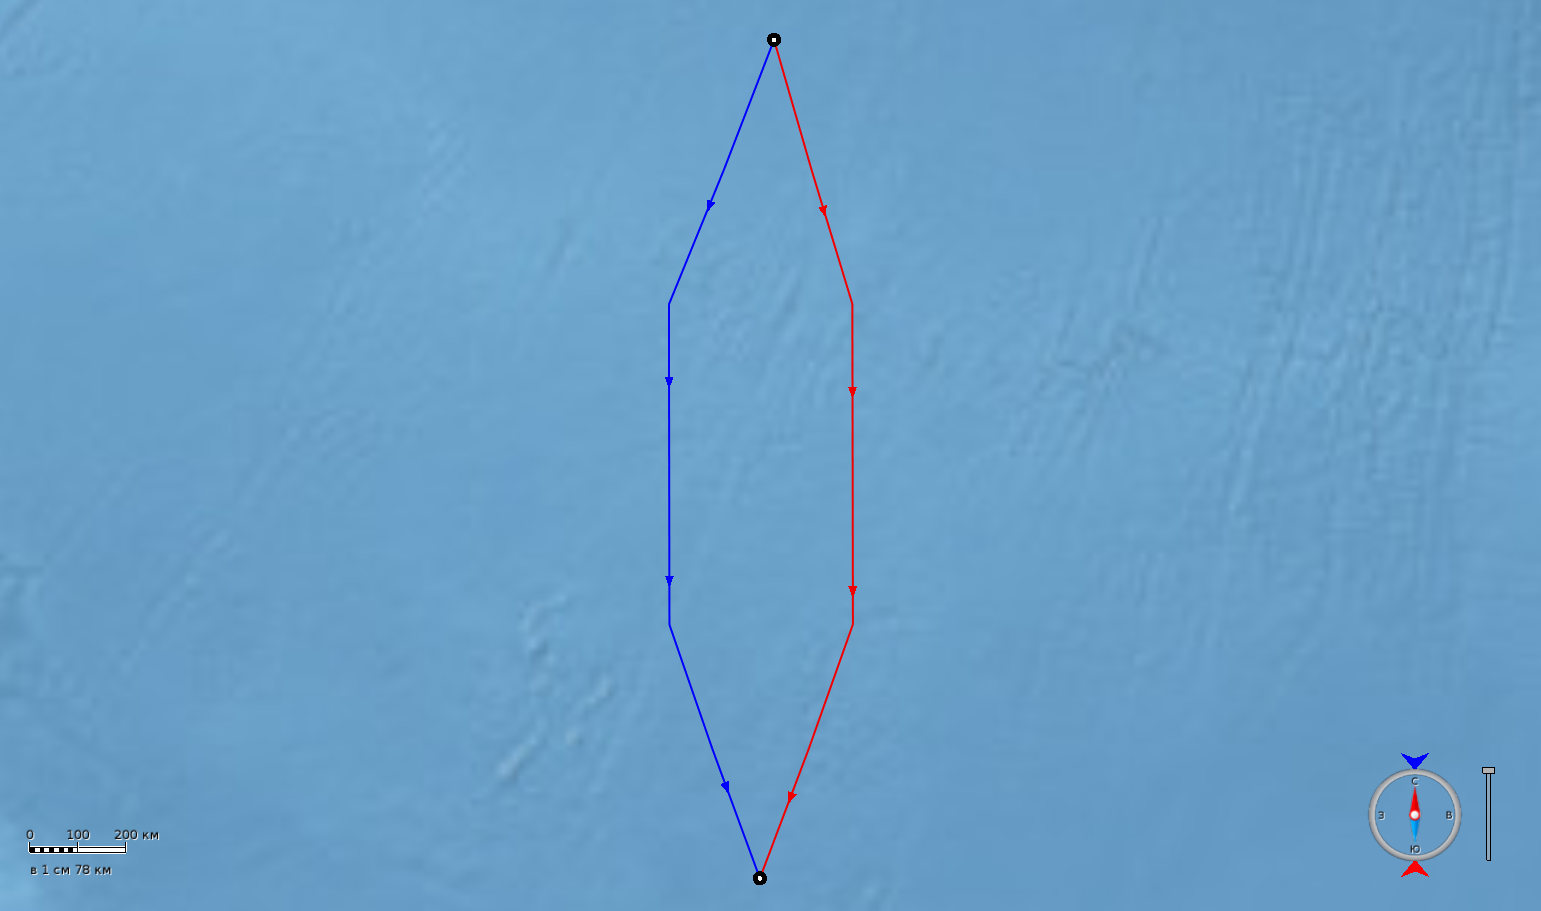
\includegraphics[width=\textwidth]{Introduction/similar}
                        
                        Похожие маршруты
                    \end{figure}
                \column{.5\textwidth}
                    \begin{figure}
                        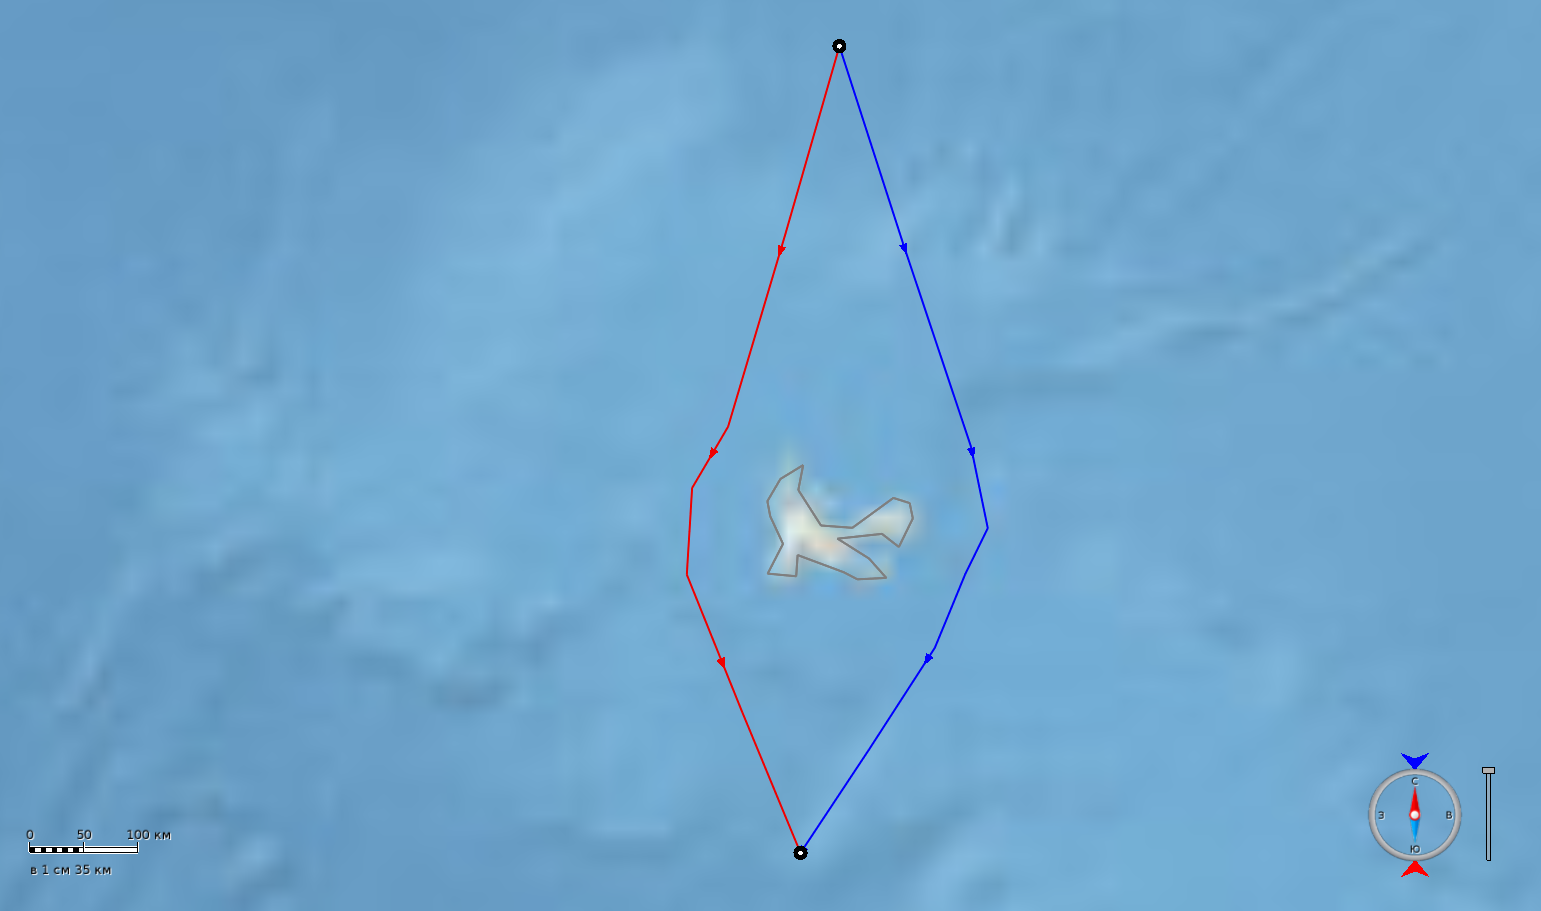
\includegraphics[width=\textwidth]{Introduction/dissimilar}

                        Непохожие маршруты
                    \end{figure}
            \end{columns}
        }
    }
    \only<4> {
        \begin{figure}
            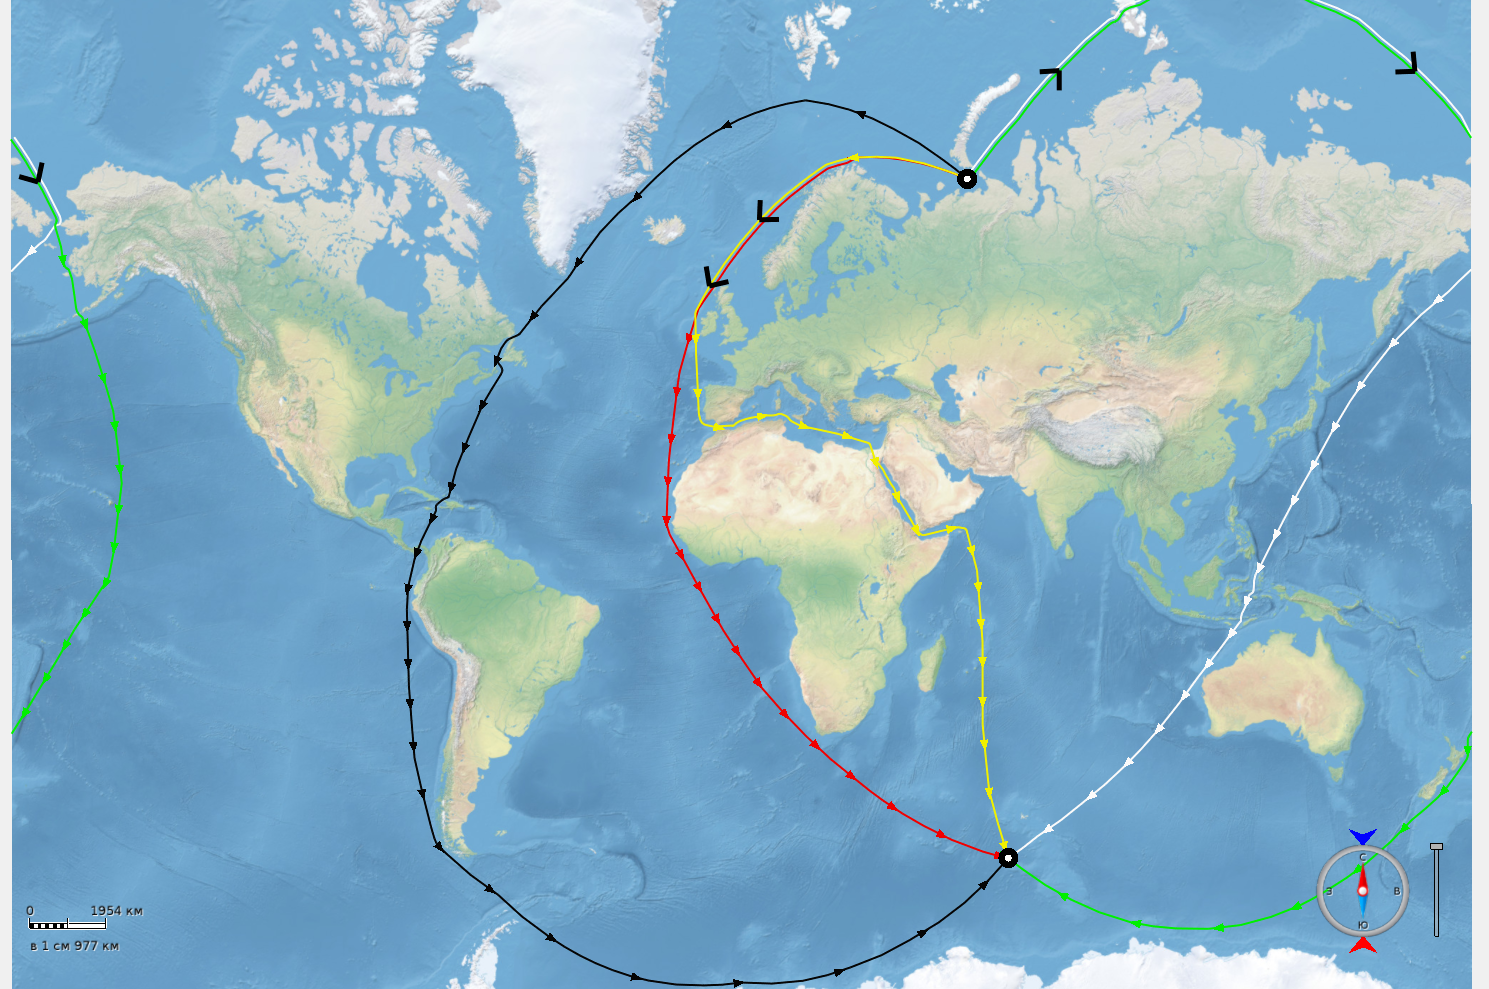
\includegraphics[width=.95\textwidth]{Introduction/my-good}

            Пример
        \end{figure}
    }
\end{frame}
\note {
Начну с неформального описания задачи. Имеется морская навигационная
карта, требуется предоставить пользователю возможность найти как можно
больше непохожих маршрутов по воде. При этом само по себе решение
задачи не является конечным результатом, а лишь поддержкой принятия
решения. Само решение принимается пользователем в голове, поэтому
основной принцип подобных задач в том, что они должны решаться в
режиме реального времени, чтобы не сбивать пользователя с мыслей.

Важно отметить, что в задаче не подразумевается поиск кратчайшего
маршрута. Суть задачи в предложении альтернативных путей.

На картинках проиллюстрировано понятие непохожести маршрутов.
}


\begin{frame}{Актуальность задачи}
    Проблемы поиска единственного маршрута:
    \begin{itemize}
        \item критерии оптимальности не всегда очевидны и формализуемы
        \item ненадёжность
     %   \item приводит к повышенной загруженности
    \end{itemize}
    \uncover<2>{Неизвестны алгоритмы multipath planning на воде}
\end{frame}
\note {
Зачем это надо?

Задача поиска кратчайшего маршрута при наличии полигональных
препятствий хорошо известна и исследована, однако при таком подходе
возникают следующие проблемы:
1. Кратчайший путь (по какой-либо метрике) не всегда оптимален, а
реальные критерии оптимальности могут быть не очевидны и трудно
формализуемы (например, стоимость прохода через канал, личные
предпочтения капитана).
% Например, где-то может быть
% платный проезд, также нужно учитывать глубину, загруженность. Также у
% капитана могут быть личные предпочтения, которые невозможно
% формализовать.

2. Если по каким-то причинам проплыть по кратчайшему маршруту не
представляется возможным (проходят учения/информация устарела/etc.),
то возникает проблема, потому что нет альтернатив.

% 3. Если приложение набирает популярность и все пользуются одинаковыми
% (например, кратчайшими) маршрутами, это может приводить повышенной загруженности.

Неизвестны алгоритмы. Тут плавный переход к следующему слайду.
}

        
\subsection{Обзор сделанного}

\begin{frame}{Существующие алгоритмы}
    \only<1> {
    Известные алгоритмы multipath planning:
    \begin{itemize}
        \item разрабатывались для других целей
        \item не учитывают реальное физическое расположение
          вершин в графе
        \item строят очень похожие маршруты на морских картах
    \end{itemize}
    }
    \only<2> {
        \begin{figure}
            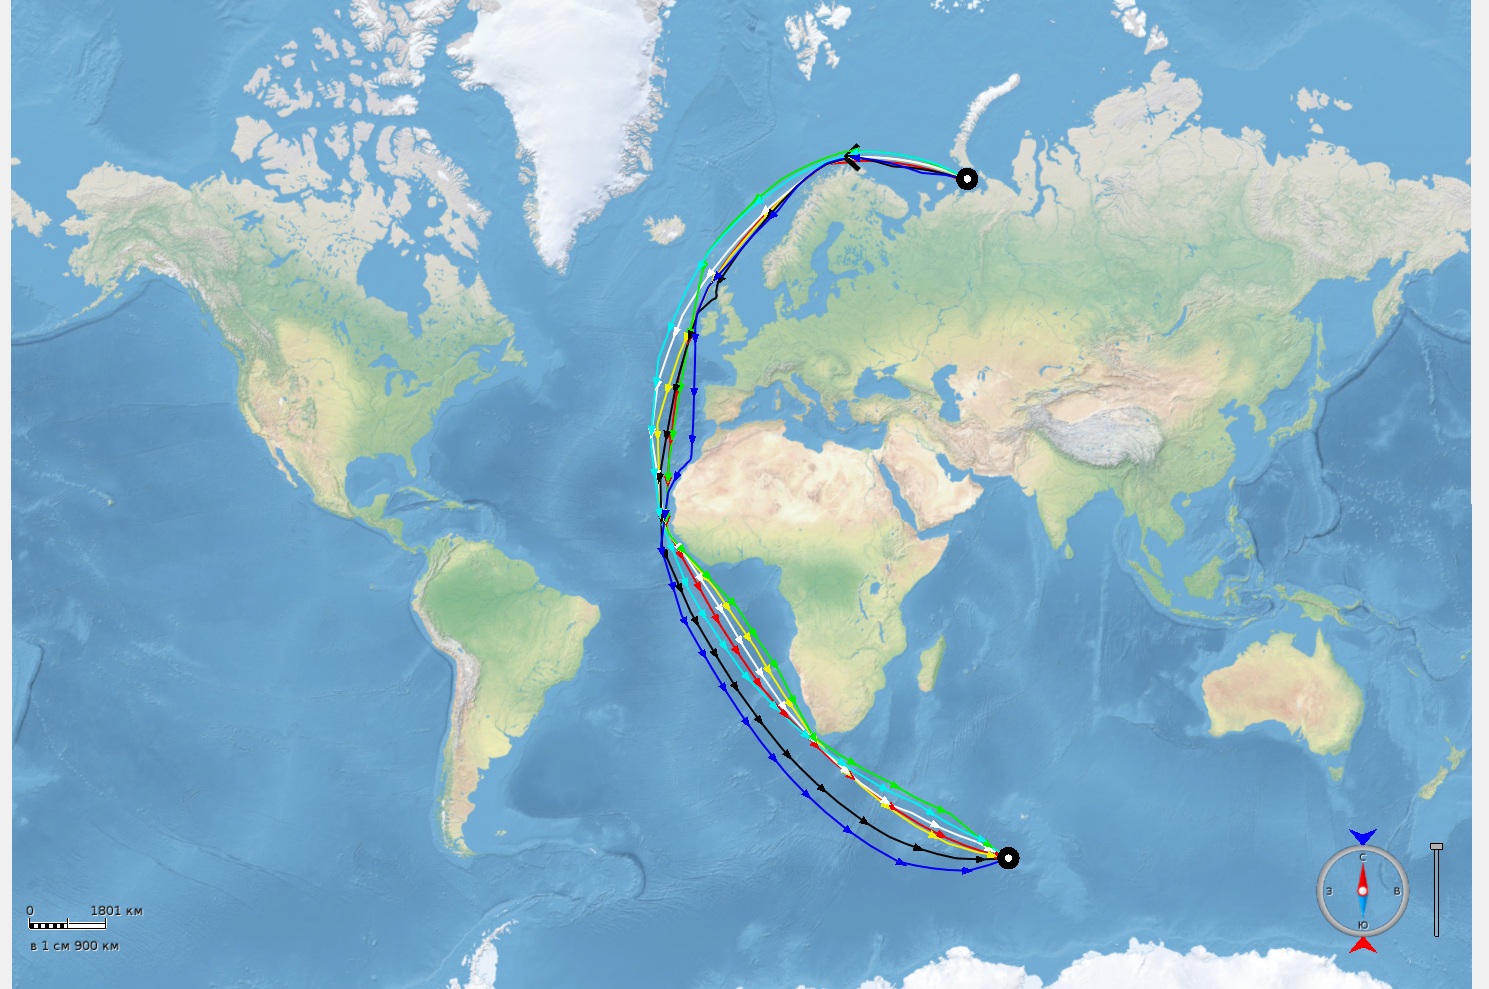
\includegraphics[width=.95\textwidth]{Introduction/existing-bad}

            Алгоритм из Yongtaek, Hyunmyung, 2005
        \end{figure}
    }
\end{frame}
\note {
Известны различные алгоритмы поиска нескольких путей в графе. Однако
все они не годятся для данной задачи.

Разрабатывались для других целей: например, поиск маршрутов по
дорогам, поиск маршрутов на общественном транспорте, когда есть
несколько способов добраться из точки А в точку Б. 

Не учитывают расположение: эти алгоритмы в большинстве своём оперируют абстрактными графами, не привязанными к конкретным координатам в мире.

Похожие маршруты: как следствие, попытка применить эти алгоритмы к
данной задаче приводит к похожим маршрутам.

Пример: видно, что маршруты почти не имеют общих рёбер, однако,
неформально говоря, они очень похожи. 
}

\subsection{Формальная постановка}

\begin{frame}{Формальная постановка}
    \begin{itemize}
        \item Дано: множество полигональных препятствий, начальная (S) и конечная (D) точки.

        \item Найти: множество путей, соединяющих точки S и D и удовлетворяющих требованиям:
        \begin{itemize}
            \item отношение длины пути к длине кратчайшего пути
              ограничено сверху константой
            \item для любых двух путей выполнен критерий непохожести
        \end{itemize}
        
        \item Время выполнения запроса: меньше секунды
    \end{itemize}
\end{frame}
\note {
Перейдём к формальной постановке задачи.

Более менее всё можно просто зачитать. Про критерий непохожести будет
сказано на следующем слайде. Поскольку требуется искать маршруты в
реальном времени, потребуем не больше секунды на запрос.
}

\begin{frame}{Метрики на маршрутах}
    \only<1> {
        \begin{equation*}
            \rho_1 (P, Q) = \max(\max_{u \in P} \min_{v \in Q} \rho_g(u,
            v), \max_{u \in Q} \min_{v \in P} \rho_g(u, v))
        \end{equation*}

        \begin{equation*}
            \rho_2 (P, Q) = \max(\max_{u \in P} \frac{\min\limits_{v \in Q_u}
            \rho_g(u, v)}{\min\limits_{v \in Q_u} \rho_r(u, v)}, \max\limits_{u \in Q} \frac{\min\limits_{v \in P_u}
            \rho_g(u, v)}{\min\limits_{v \in P_u} \rho_r(u, v)})
        \end{equation*}
        
        \begin{equation*}
            Q_u = \{ v : \rho_r(u, v) > \varepsilon \}
        \end{equation*}
    }
    \only<2> {
        \begin{figure}
            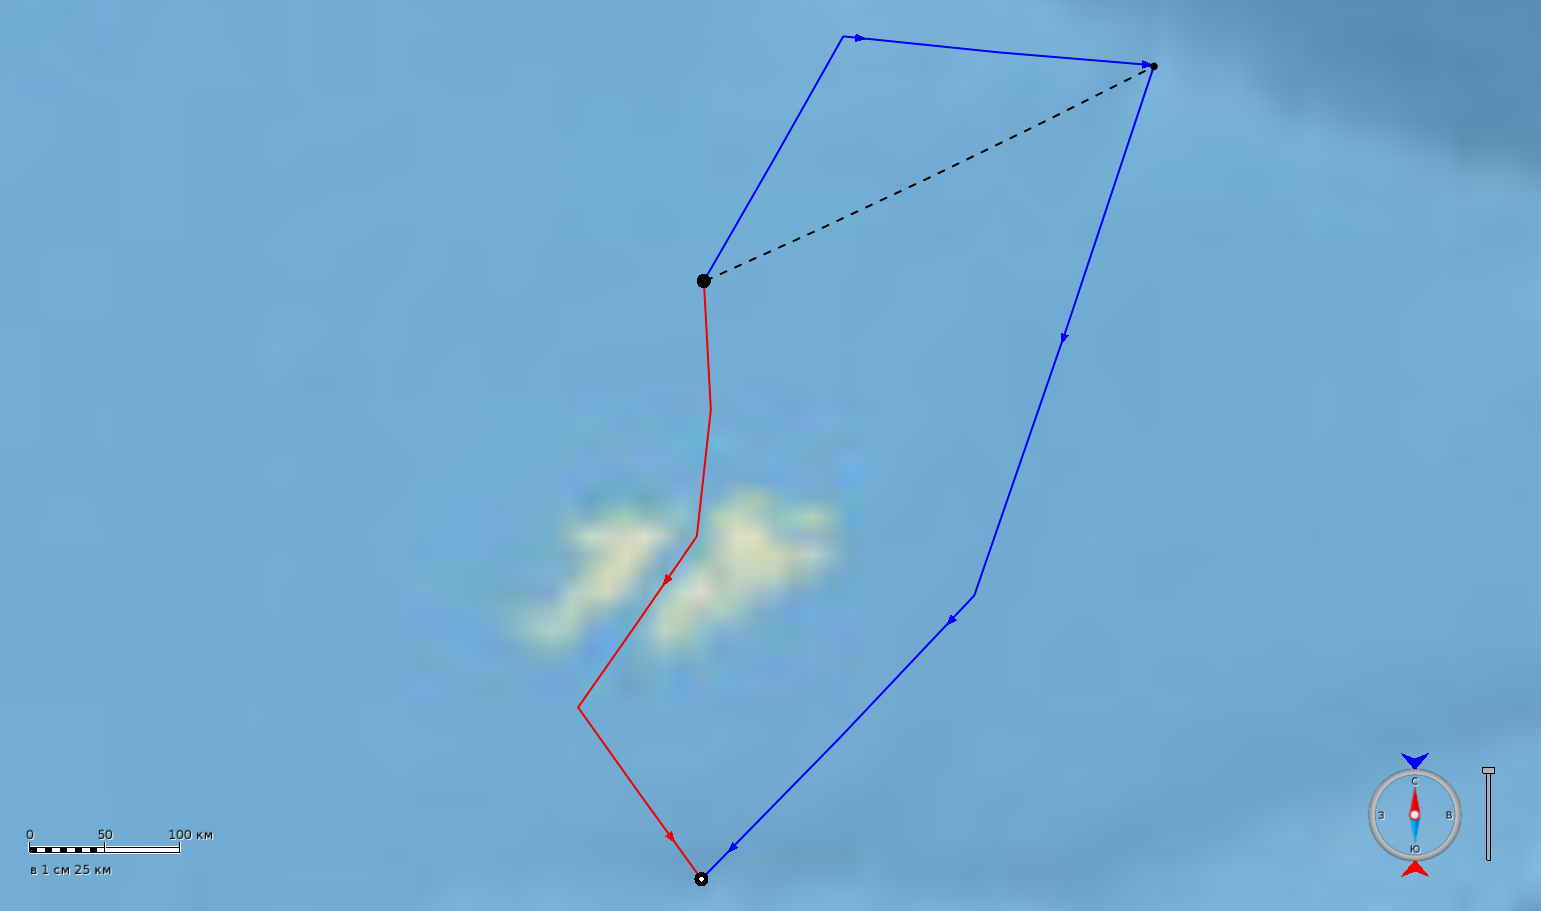
\includegraphics[width=.95\textwidth]{Solution/metrics/1-dissimilar}
            
            $\frac{\rho_1}{l_{min}} = \frac{339}{435} = 0.78$
        \end{figure}
    }
    \only<3> {
        \begin{figure}
            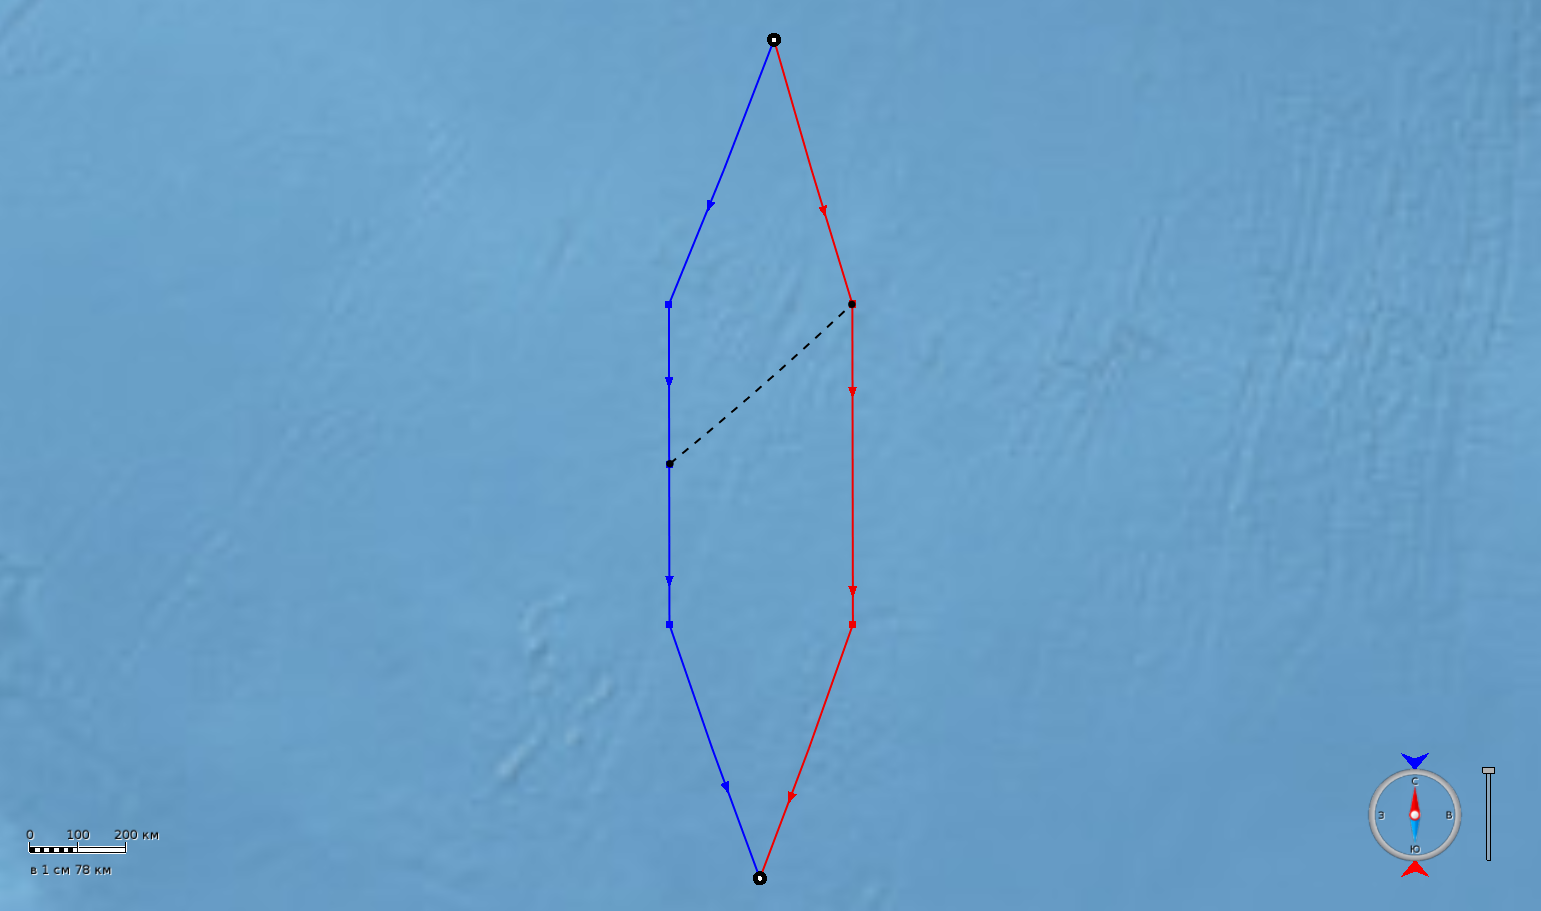
\includegraphics[width=.9\textwidth]{Solution/metrics/1-uncertain-2-similar}
            
            $\frac{\rho_1}{l_{min}} = \frac{502}{1704} = 0.29$

            $\rho_2 = 1$
        \end{figure}
    }
    \only<4> {
        \begin{figure}
            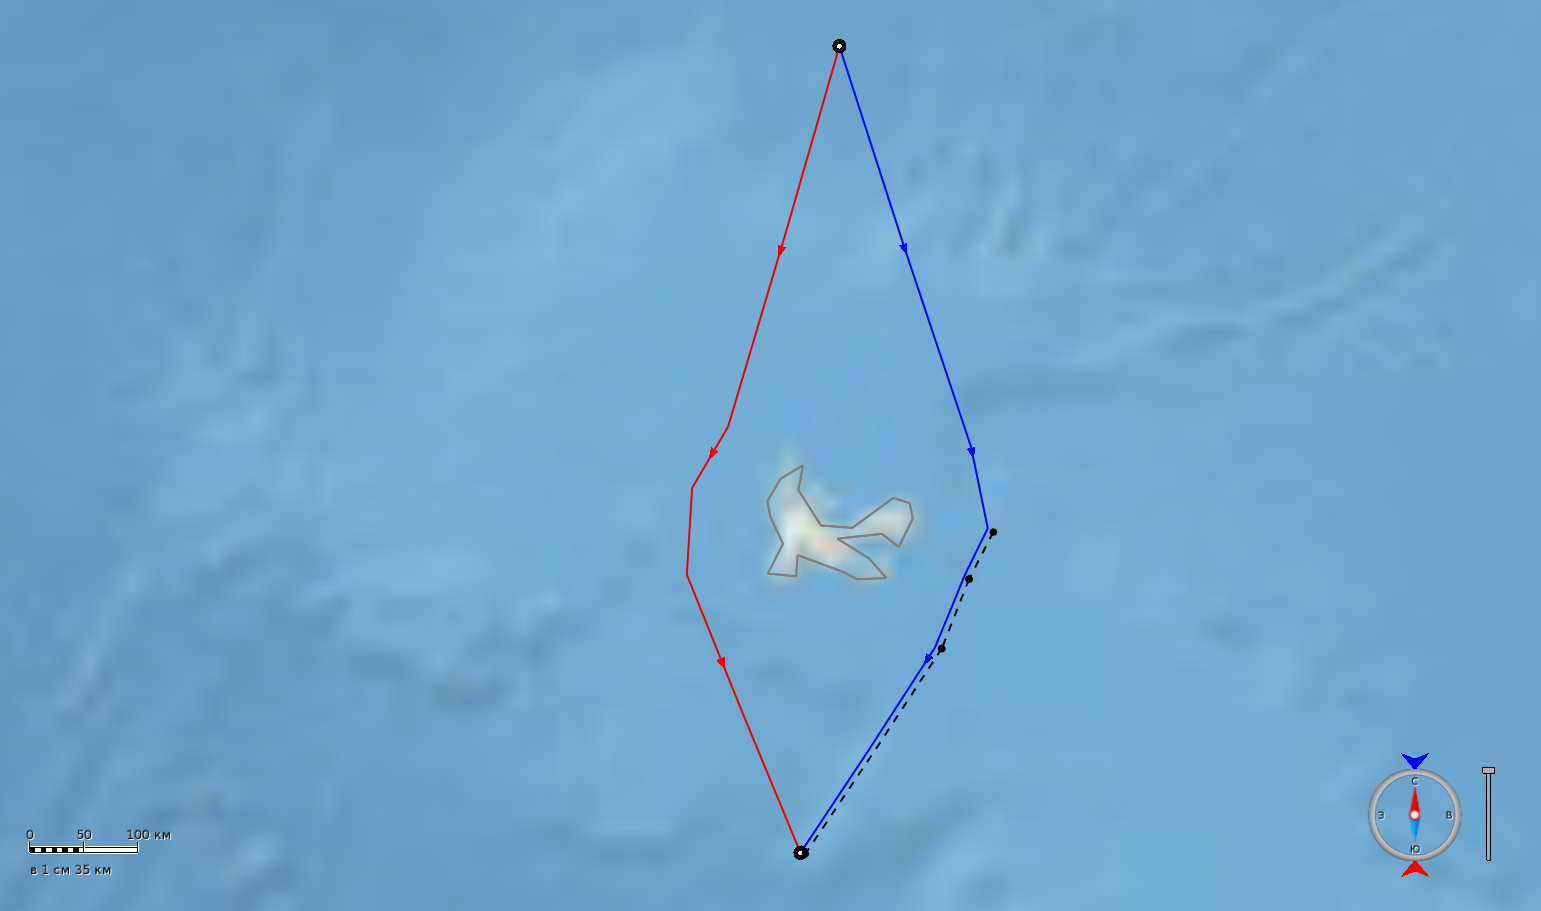
\includegraphics[width=.95\textwidth]{Solution/metrics/1-uncertain-2-dissimilar-gclosest}
            
            $\frac{\rho_1}{l_{min}} = \frac{331}{781} = 0.42$
        \end{figure}
    }
    \only<5> {
        \begin{figure}
            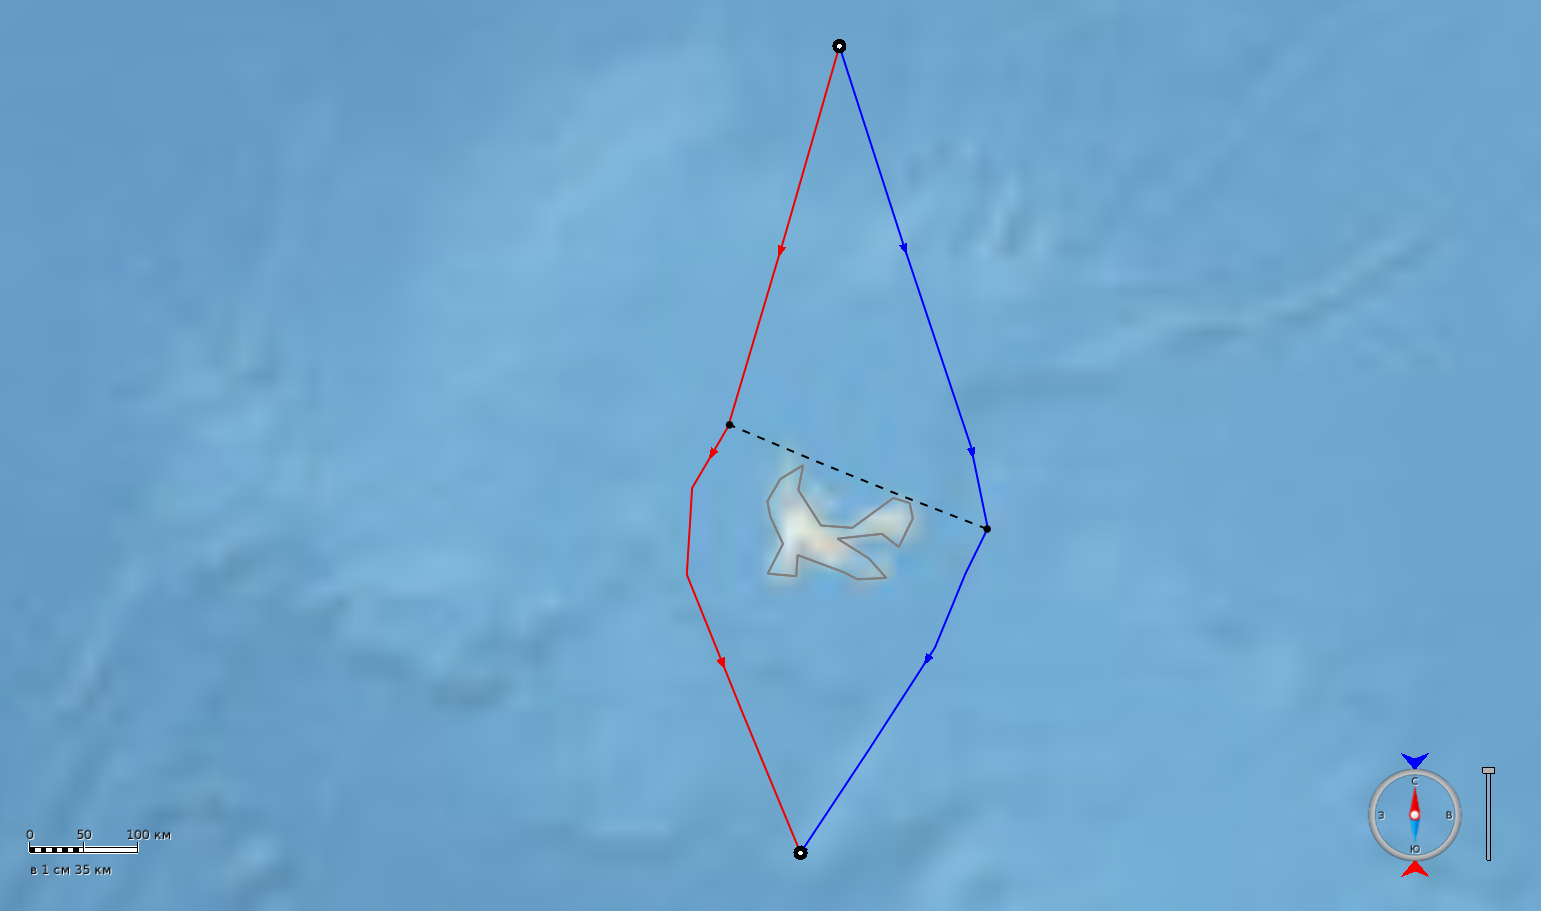
\includegraphics[width=.9\textwidth]{Solution/metrics/1-uncertain-2-dissimilar-closest}
            
            $\frac{\rho_1}{l_{min}} = \frac{331}{781} = 0.42$

            $\rho_2 = \frac{331}{255} = 1.3$
        \end{figure}
    }
    \only<6> {
        \begin{figure}
            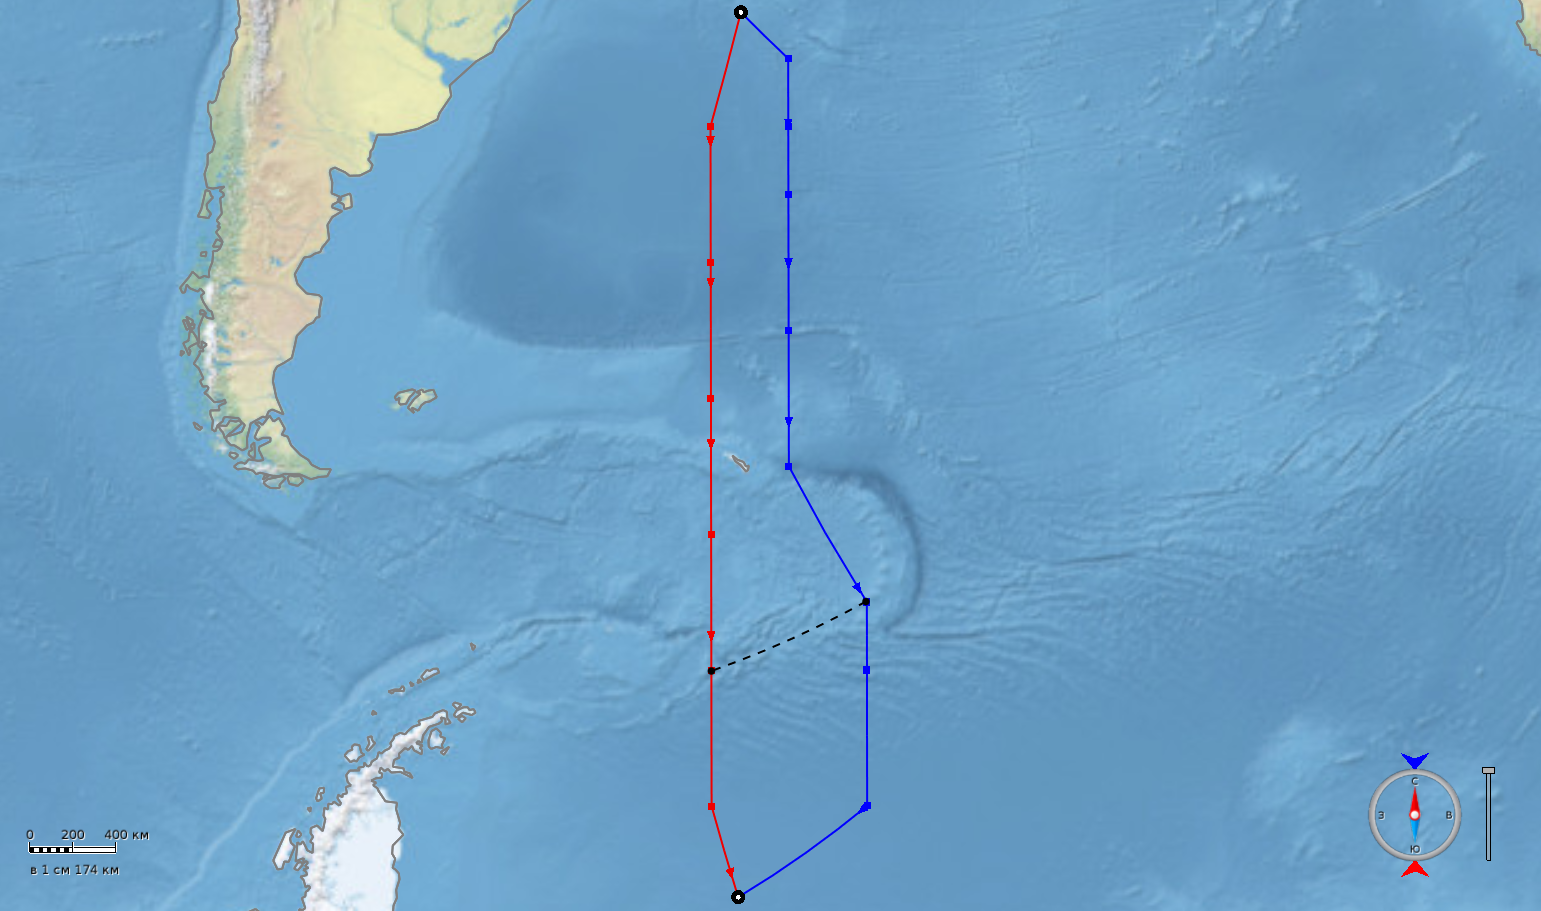
\includegraphics[width=.95\textwidth]{Solution/metrics/1-similar}
            
            $\frac{\rho_1}{l_{min}} = \frac{641}{4059} = 0.16$
        \end{figure}
    }
\end{frame}
\note {
Сначала сказать, что такое $\rho_g$ и $\rho_r$.

Первая метрика берёт для каждой вершины первого пути расстояние до
ближайшей вершины второго пути и находит максимум этих расстояний.
В зависимости от отношения её значения к длине кратчайшего из двух
путей маршруты считаются либо похожими, либо непохожими, либо
«возможно, похожими». В последнем случае используется вторая метрика.

Вторая метрика аналогична первой, но графовое расстояние до ближайшей
вершины в графе делится на реальное расстояние до ближайшей вершины в
мире. Большое значение этой метрики означает, что между путями есть
какое-то препятствие. При этом не рассматриваются слишком близкие
вершины, поскольку между ними может быть незначительное препятствие.

}

\section{Решение}

\subsection{Предобработка}

\begin{frame}{Предобработка данных}
    \begin{itemize}
        \item Карта → полигон
        \item Смещение полигона внутрь
        \item Граф по сетке на плоскости + граф локальной видимости
        \item Ограничение длины ребра
        \item Дополнительные рёбра
    \end{itemize}
\end{frame}
\note {
1. Склеивание, упрощение. Полигон — множество контуров (в том числе дырок).

2. Полигон смещается внутрь, потому что, во-первых, корабли не плавают
слишком близко к суше, а во-вторых, так будут лучше видны маршруты.
Используется straight skeleton.

3. Чтобы находить кратчайший путь, нужен граф видимости. Но в нём
слишком много рёбер, поэтому построим навигационный граф. Разложим
вершины по сетке, проведём рёбра до соседей (и их соседей). Также
добавим вершины полигона и проведём из них рёбра до ближайших видимых 
вершин. Веса рёбер — расстояния между точками на сфере.

4. Путь ищется на сфере, при этом проверка корректности рёбер
осуществляется на плоскости. Кратчайшая траектория на сфере отличается
от кратчайшей траектории на плоскости. Не будем допускать слишком
длинные рёбра, тогда расхождение будет пренебрежимо мало.

5. Во-первых, добавим рёбра из straight skeleton'а, получившиеся в
результате схлопывания. Во-вторых, нужна возможность добавления рёбер
в связи с неточностями исходной карты. В-третьих, рёбра через 180-ый меридиан.
}

\subsection{Основы поиска}

\begin{frame}{Поиск одного маршрута}
    \only<1-4> {
        \begin{itemize}
            \item<1-4> Добавление вершин в граф
            \item<2-4> Алгоритм Дейкстры
            \item<3-4> Сокращение маршрута
            \begin{itemize}
                \item<3-4> Если подпуть A → B → C можно выгодно заменить на A → C, заменяем 
                \item<3-4> Подразбиение маршрута
            \end{itemize}
            \item<4-4> Сглаживание маршрута
        \end{itemize}
    }
    \only<5> {
        \begin{figure}
            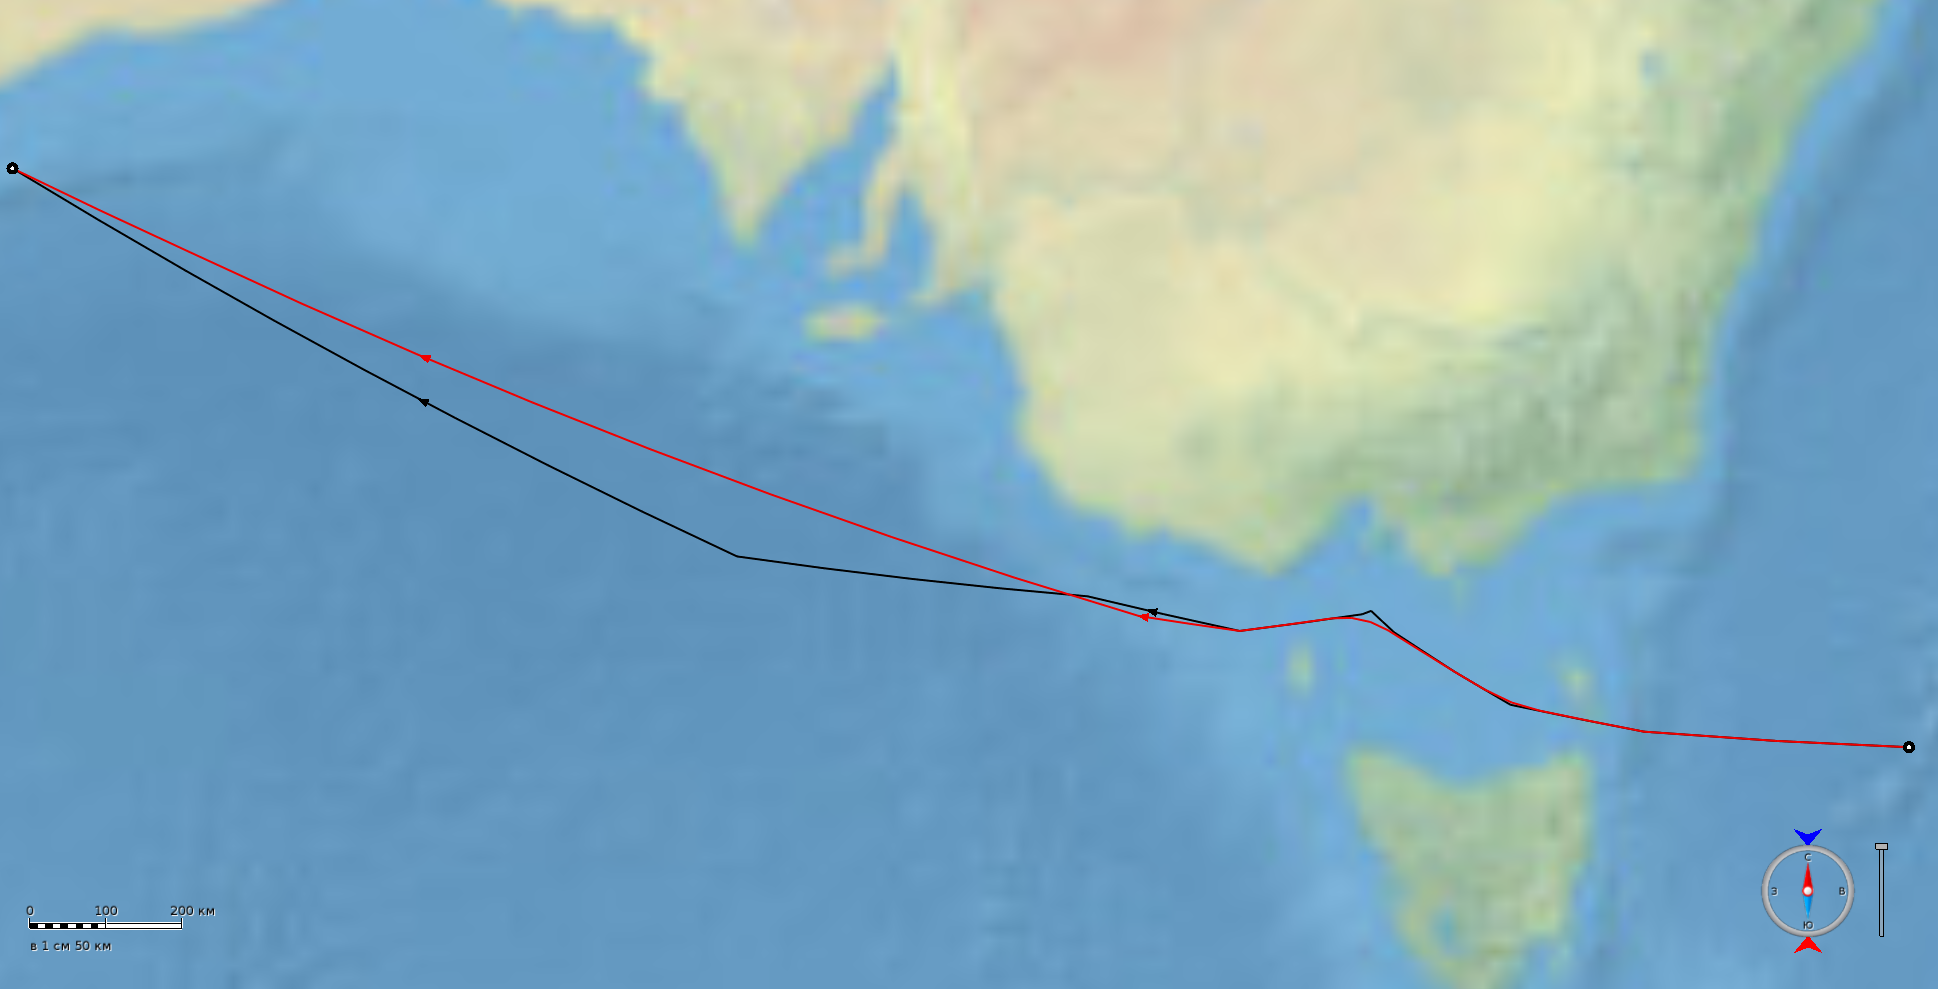
\includegraphics[width=\textwidth]{Solution/shortcut-and-smoothing}
            
            Сокращение и сглаживание
        \end{figure}
    }
\end{frame}
\note {
% Добавление вершин: проверяем, принадлежит ли воде. Добавляем вершину в граф. По сетке находим ближайшие вершины и добавляем к ним рёбра.
Перейдём к описанию алгоритма. Начнём с описания поиска одного
маршрута, поскольку он лежит в основе поиска семейств маршрутов.

С помощью имеющихся библиотек читается карта, происходит упрощение
геометрии и склеивание контуров, в результате получается полигон,
который смещается внутрь, поскольку корабли не плавают слишком близко
к суше. Затем строится регулярная сетка, её рёбра, принадлежащие
полигону,  добавляются в навигационный граф, также добавляются рёбра
графа локальной видимости, то есть графа видимости с ограничением длины ребра.

Алгоритм Дейкстры: очевидно.

Сокращение маршрута: кратчайший путь в навигационном графе не обязан
быть действительно кратчайшим путём. Обычно его можно сократить.

Сглаживание: в связи со структурой графа возможно появление слишком
острых углов в маршруте, которые выглядят неестественно, поэтому
выполняется их сглаживание.
}

\end{document}

\subsection{Поиск нескольких маршрутов}

\begin{frame}{Поиск нескольких маршрутов}
    \begin{itemize}
        \item Поиск одного маршрута
          \pause
        \item Обновление весов:
        \begin{itemize}
            \item Потенциалы как функция кратчайших расстояний от фиктивной вершины
            \item Обновление потенциалов
            \item Применение потенциалов
        \end{itemize}
          \pause
        \item Проверка критерия остановки:
        \begin{itemize}
            \item Длина маршрута
            \item Метрики на маршрутах
        \end{itemize}
    \end{itemize}
\end{frame}
\note {
Для поиска нескольких маршрутов используется итеративный алгоритм.

Поиск одного маршрута: как сказано на прошлом слайде.

Обновление весов:

После поиска одного маршрута происходит обновление весеов рёбер.

— в граф добавляется фиктивная вершина, из которой проводим рёбра нулевого веса во все вершины
пути. Запускаем алгоритм Дейкстры из фиктивной вершины, находим все
кратчайшие расстояния в некотором радиусе. Потенциал — эвристическая функция найденного
кратчайшего расстояния, определённая для каждой вершины. Чем больше
потенциал, тем сильнее нужно увеличить веса инцедентных вершине рёбер,
поэтому чем больше расстояние, тем меньше потенциал.

— затем происходит обновление потенциалов, то есть расчёт новых
потенциалов на основе имеющихся и посчитанных на текущей итерации.

— применение потенциалов состоит в модификации весов в соответствии с
потенциалами.

Критерий остановки: определяем, хороший ли маршрут. Если хороший, то
переходим к следующей итерации, иначе прекращаем.

— длина: если сильно длинее кратчайшего, то плохой.

— метрики: оцениваем похожесть на другие маршруты. Если есть похожий, то плохо.
}

\begin{frame}{Обновление весов}
    \only<1> {
        \begin{figure}
            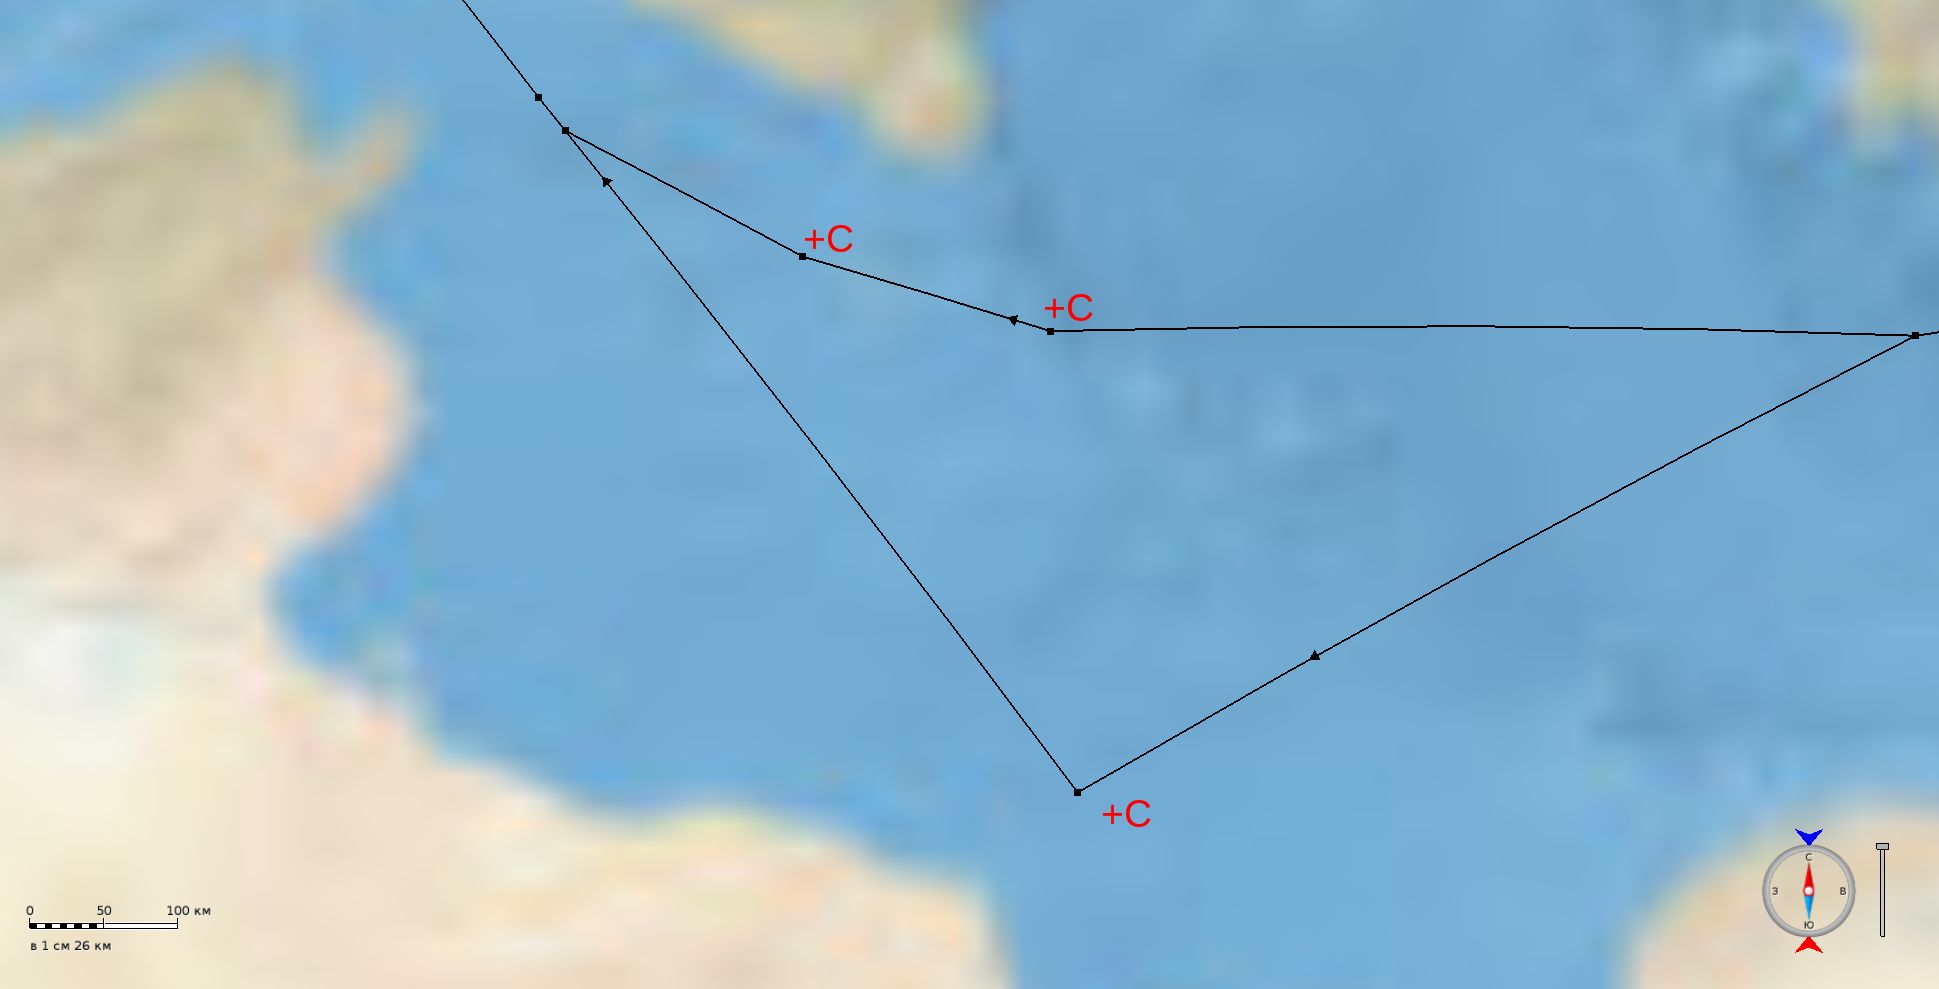
\includegraphics[width=\textwidth]{potentials-multipliers}

            Потенциалы должны быть множителями, а не слагаемыми
        \end{figure}
    }
 
    \only<2> {
        \begin{columns}
            \column{.5\textwidth}
            \begin{figure}
                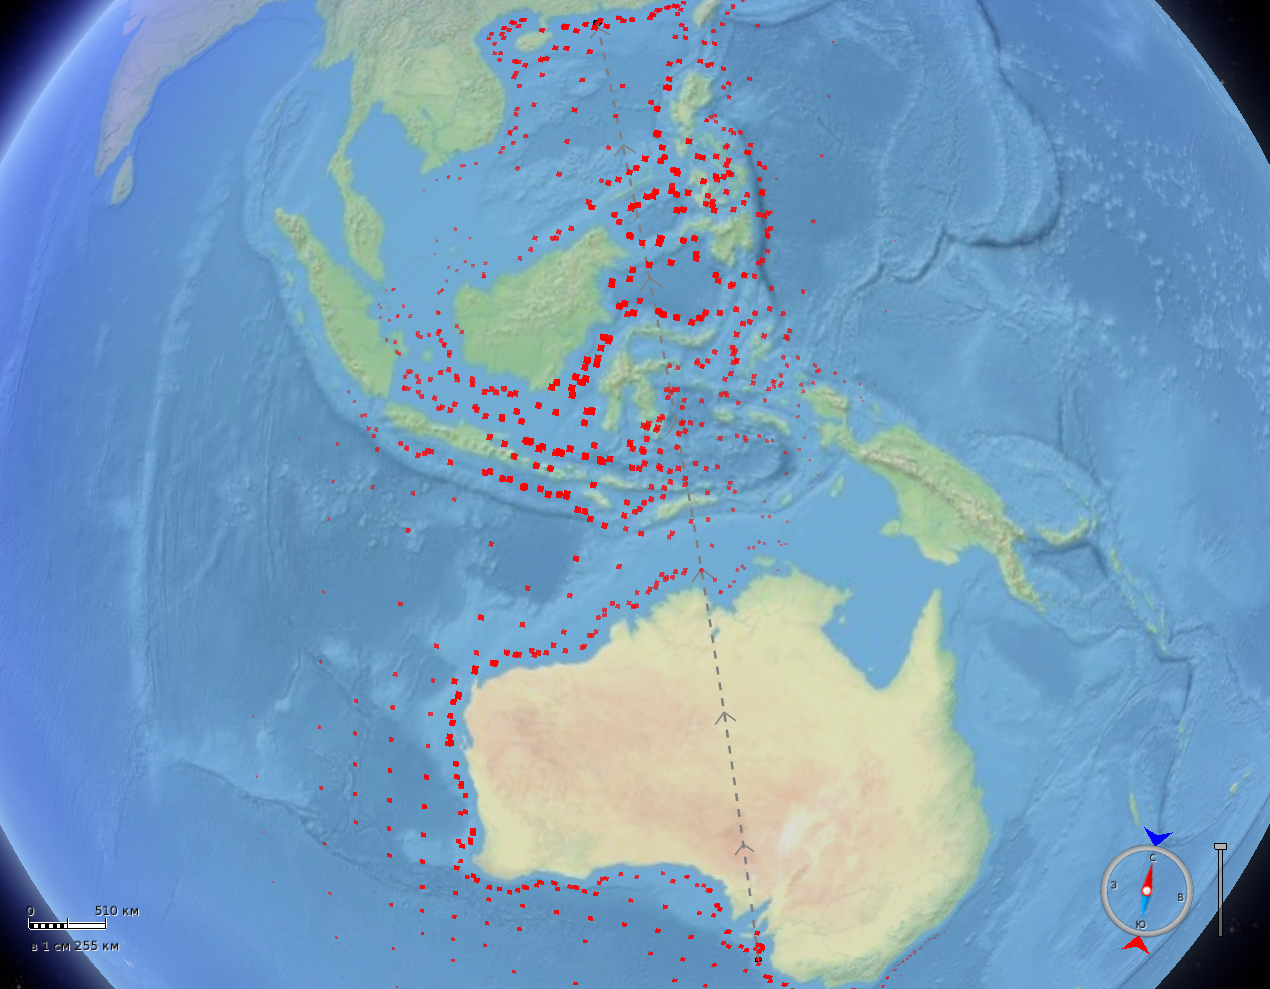
\includegraphics[clip=true, trim = 280pt 0 20pt 0, width=\textwidth]{potentials-update/accum1}
            \end{figure}

            \column{.5\textwidth}
            \begin{figure}
                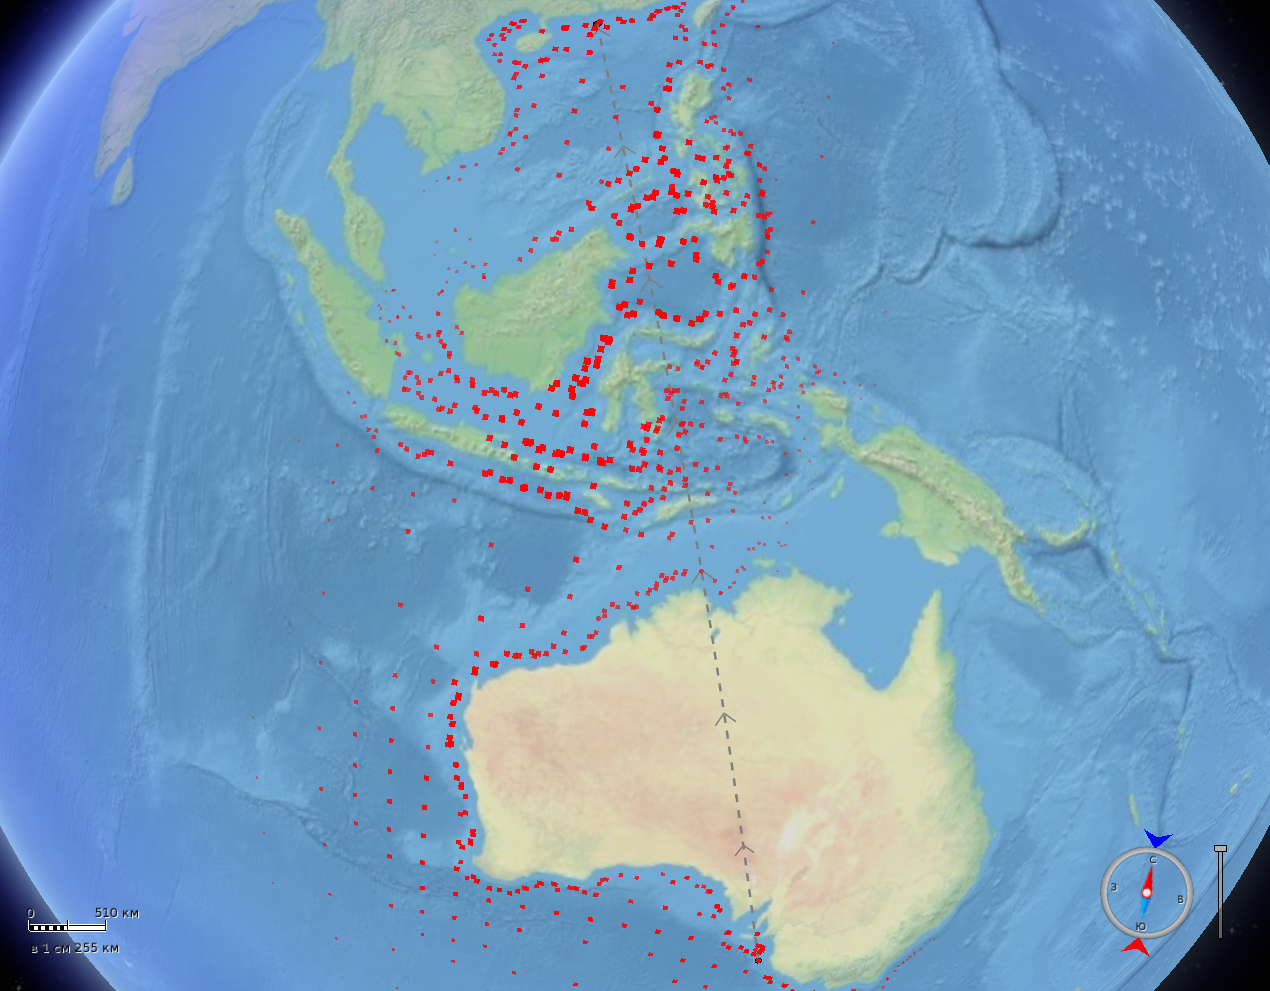
\includegraphics[clip=true, trim = 280pt 0 20pt 0, width=\textwidth]{potentials-update/max1}
            \end{figure}
        \end{columns}

        \begin{center}
            При обновлении потенциалов следует брать максимум.
        \end{center}
    }
   
    \only<3> {
        \begin{columns}
            \column{.5\textwidth}
            \begin{figure}
                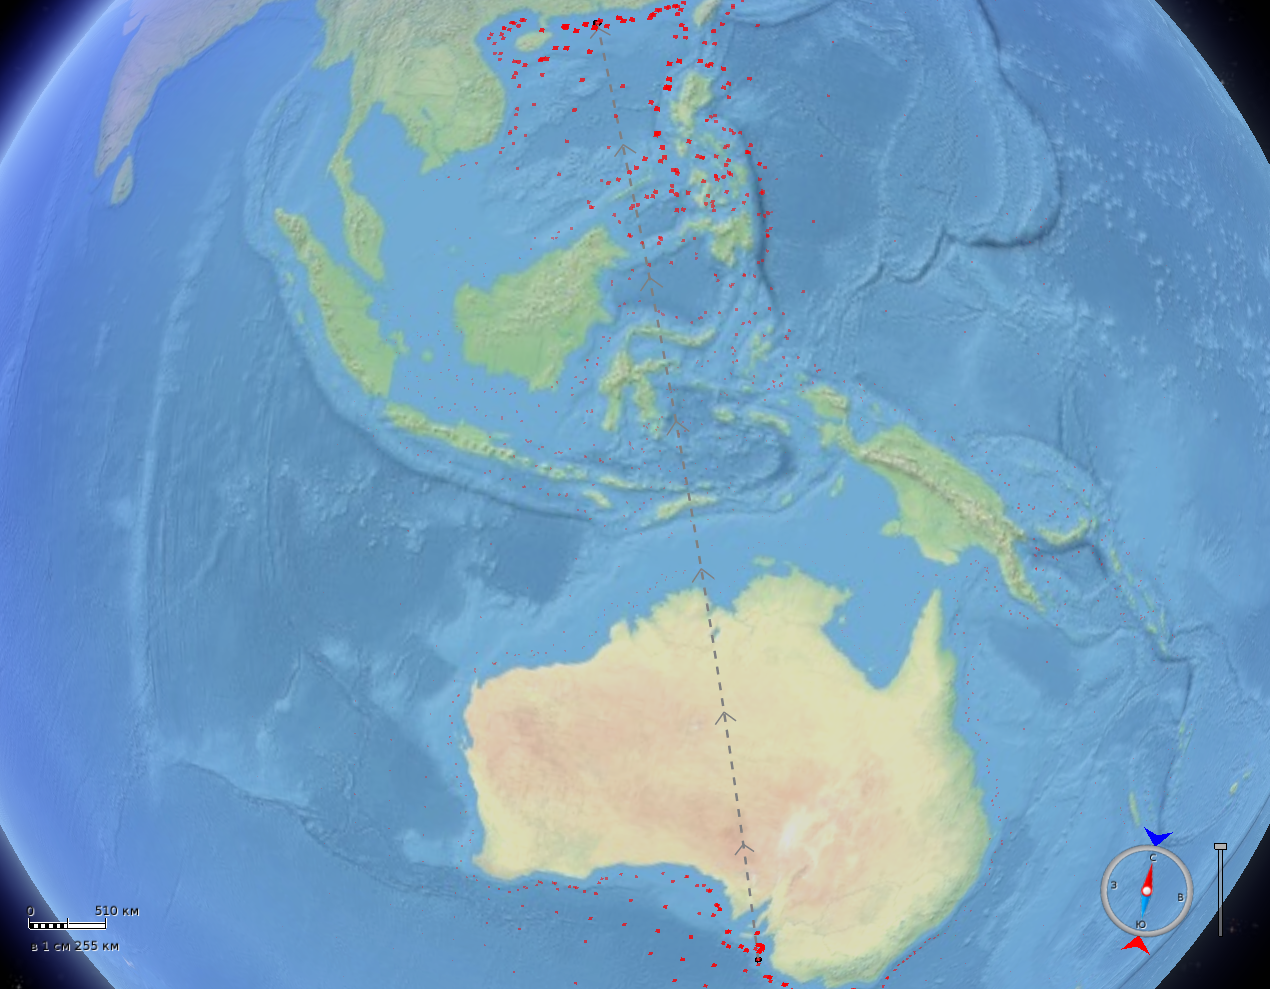
\includegraphics[clip=true, trim = 280pt 0 20pt 0, width=\textwidth]{potentials-update/accum2}
            \end{figure}

            \column{.5\textwidth}
            \begin{figure}
                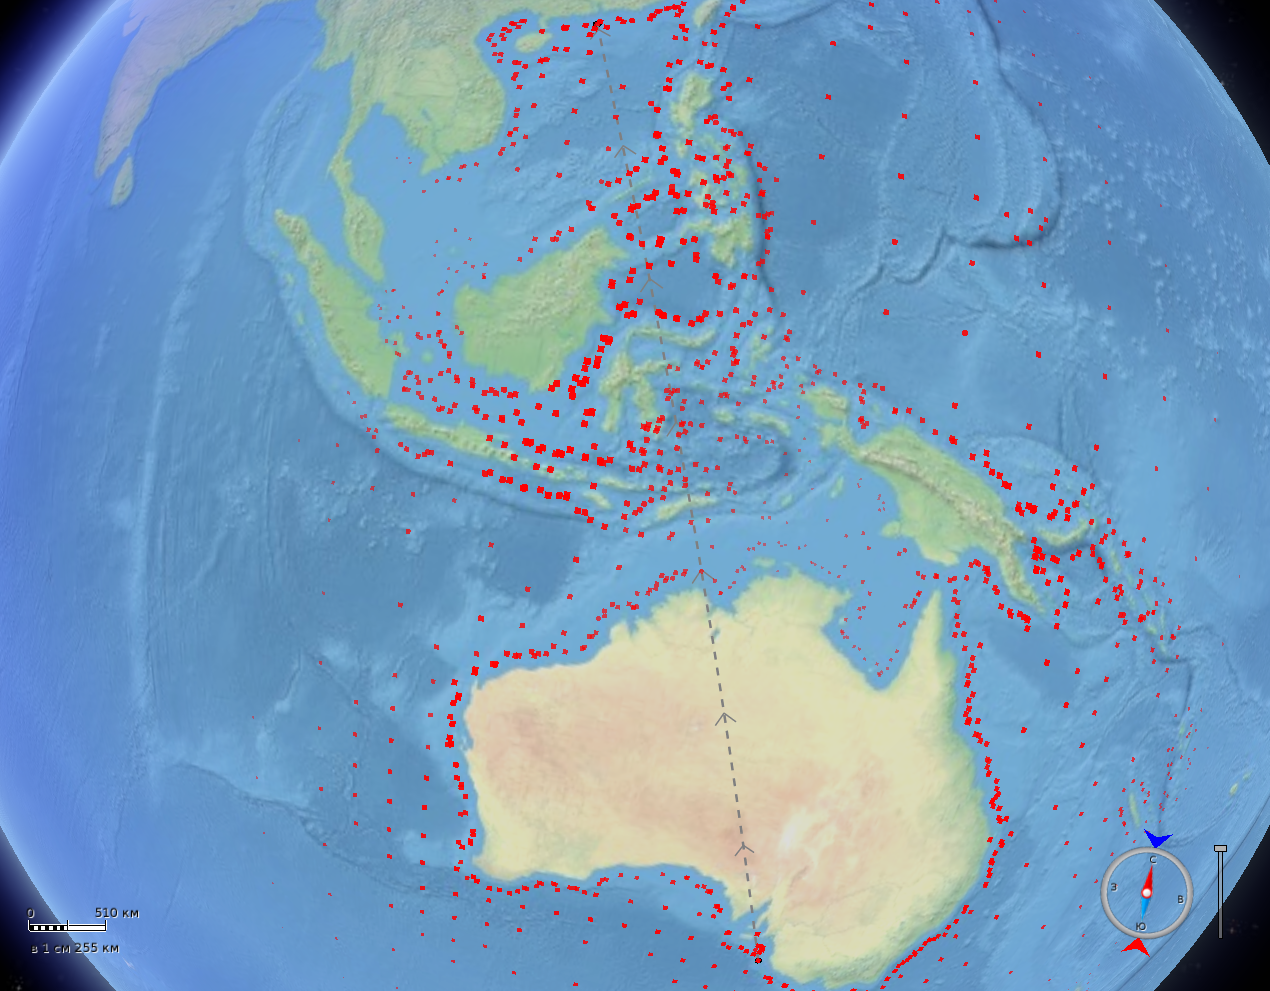
\includegraphics[clip=true, trim = 280pt 0 20pt 0, width=\textwidth]{potentials-update/max2}
            \end{figure}
        \end{columns}

        \begin{center}
            При обновлении потенциалов следует брать максимум.
        \end{center}
    }
   
    \only<4> {
        \begin{columns}
            \column{.5\textwidth}
            \begin{figure}
                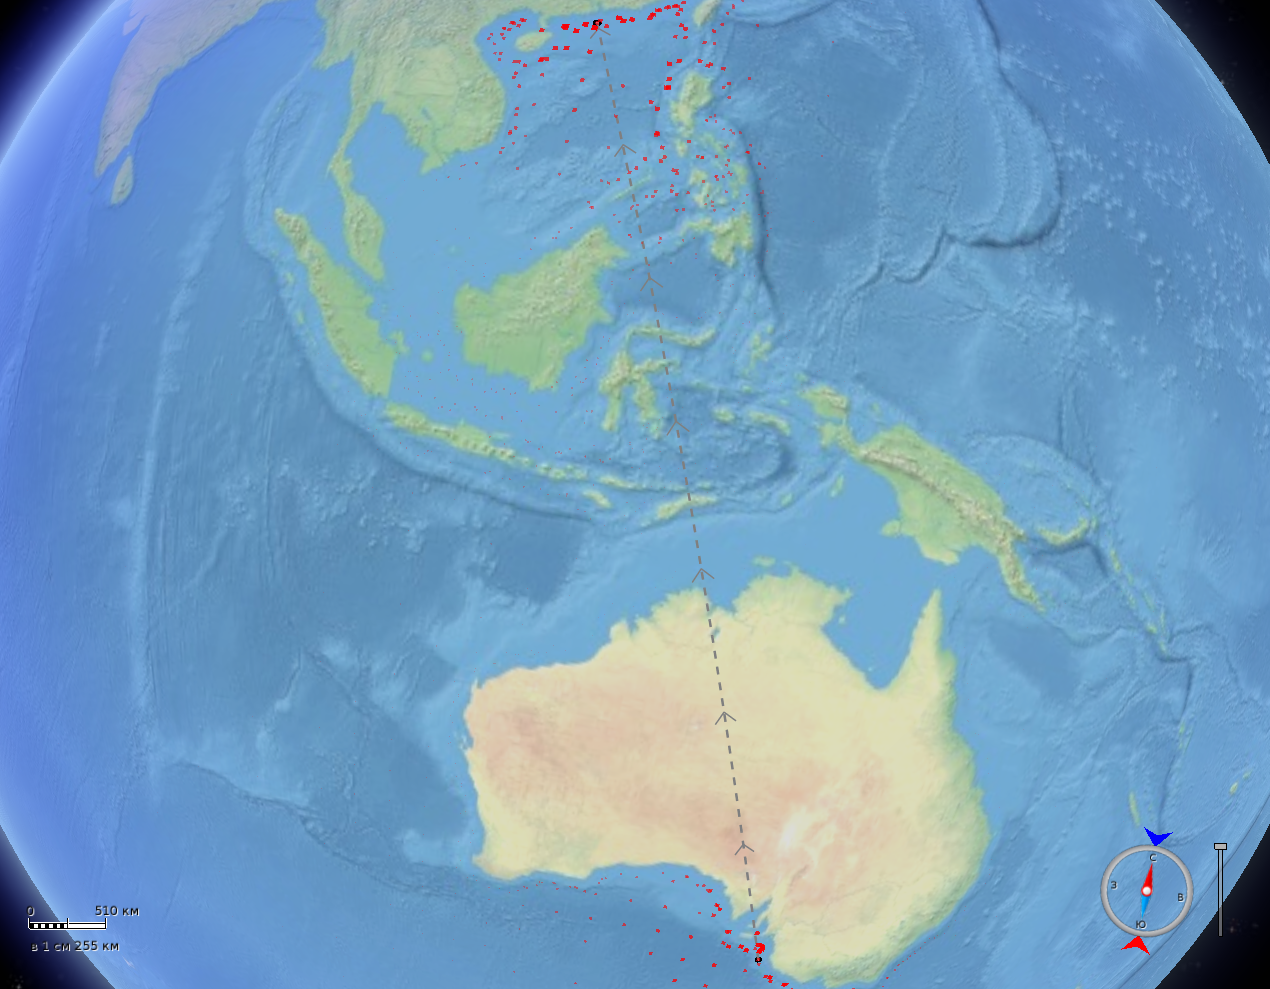
\includegraphics[clip=true, trim = 280pt 0 20pt 0, width=\textwidth]{potentials-update/accum3}
            \end{figure}

            \column{.5\textwidth}
            \begin{figure}
                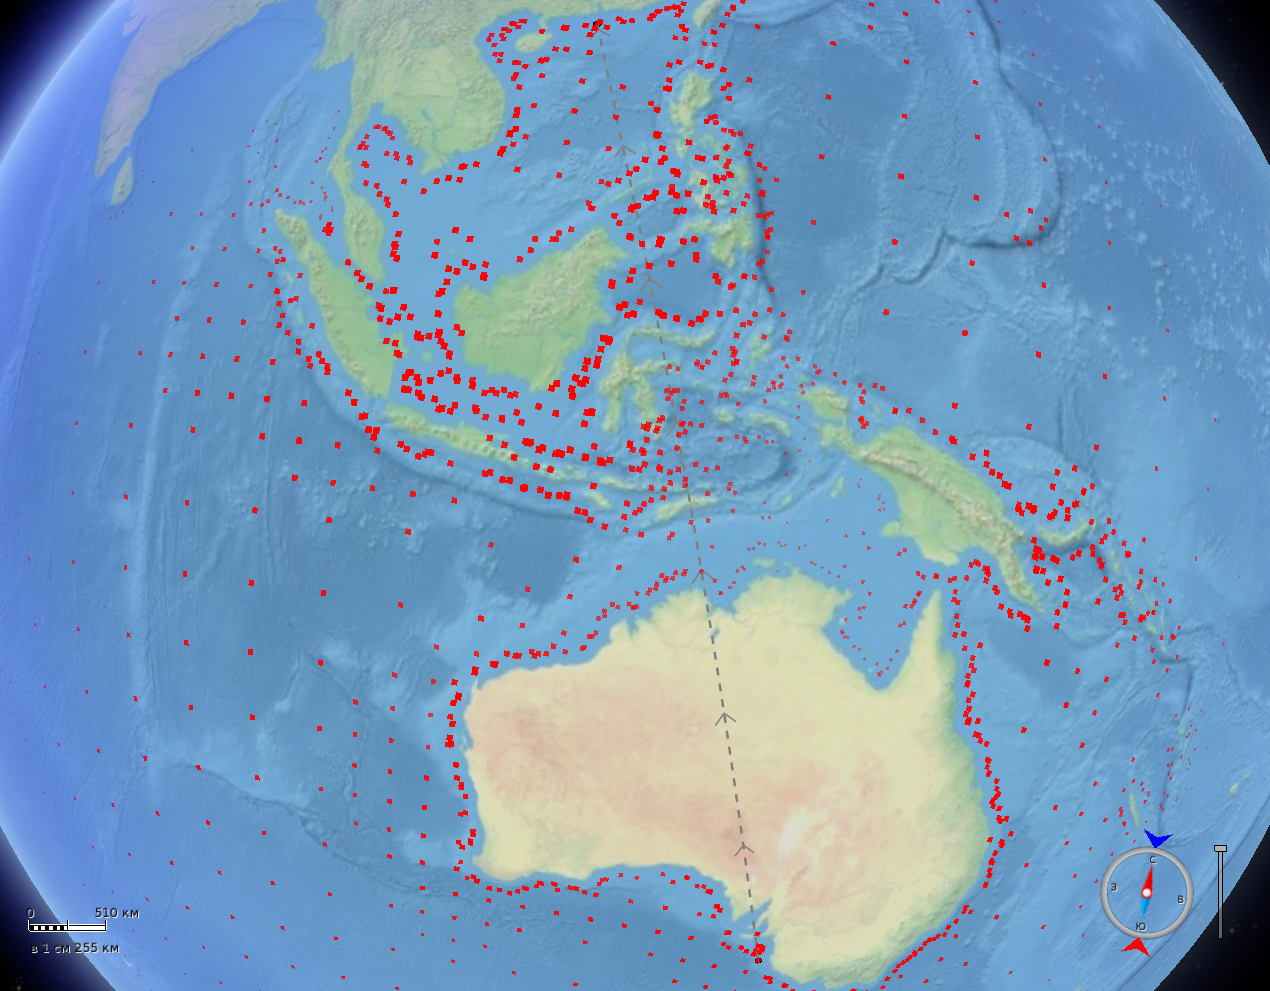
\includegraphics[clip=true, trim = 280pt 0 20pt 0, width=\textwidth]{potentials-update/max3}
            \end{figure}
        \end{columns}
        
        \begin{center}
            При обновлении потенциалов следует брать максимум.
        \end{center}
    }
   
    \only<5> {
        \begin{columns}
            \column{.5\textwidth}
            \begin{figure}
                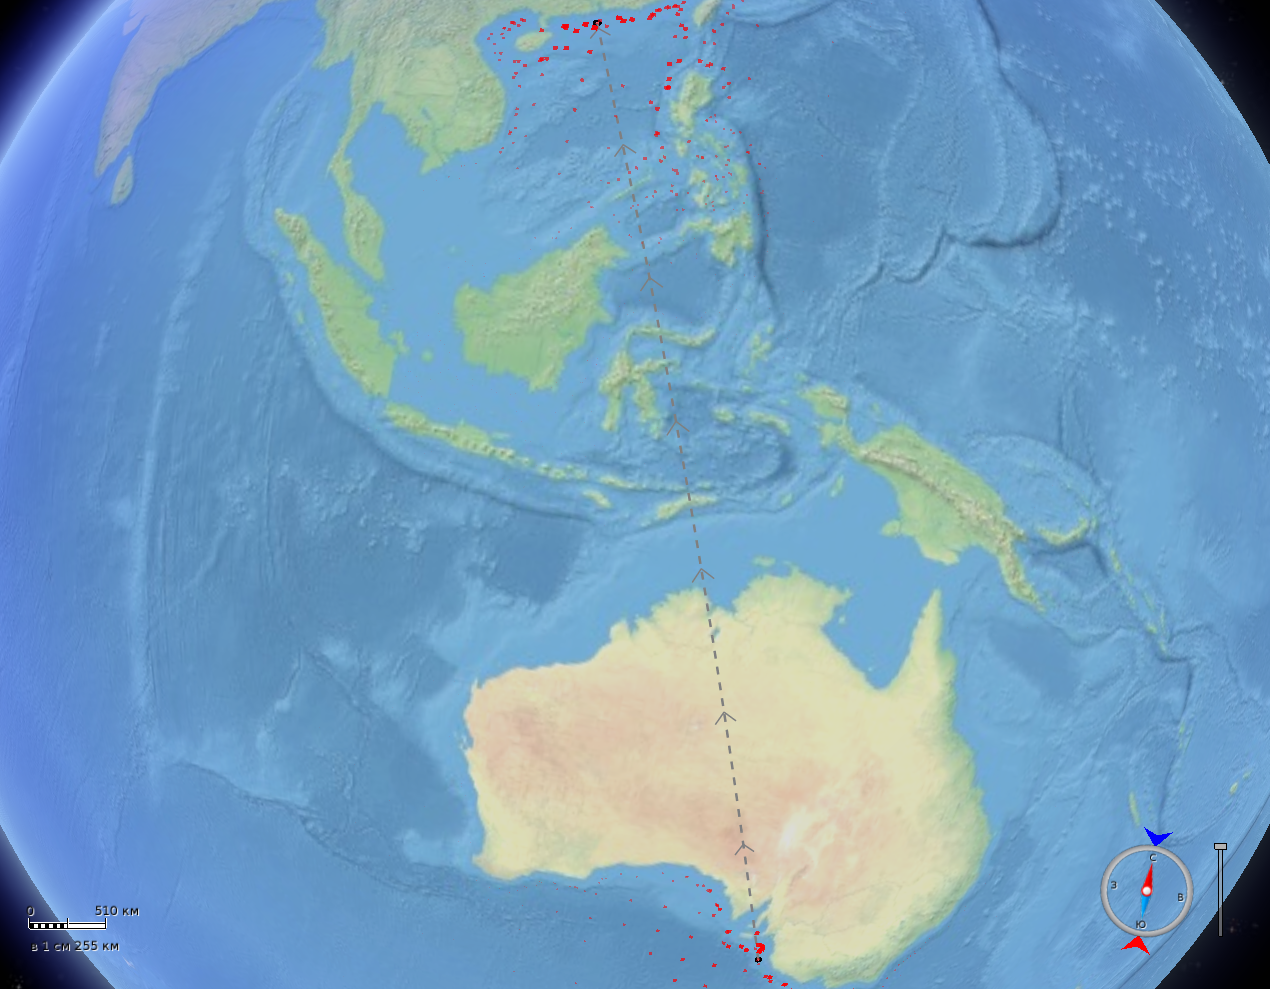
\includegraphics[clip=true, trim = 280pt 0 20pt 0, width=\textwidth]{potentials-update/accum4}
            \end{figure}

            \column{.5\textwidth}
            \begin{figure}
                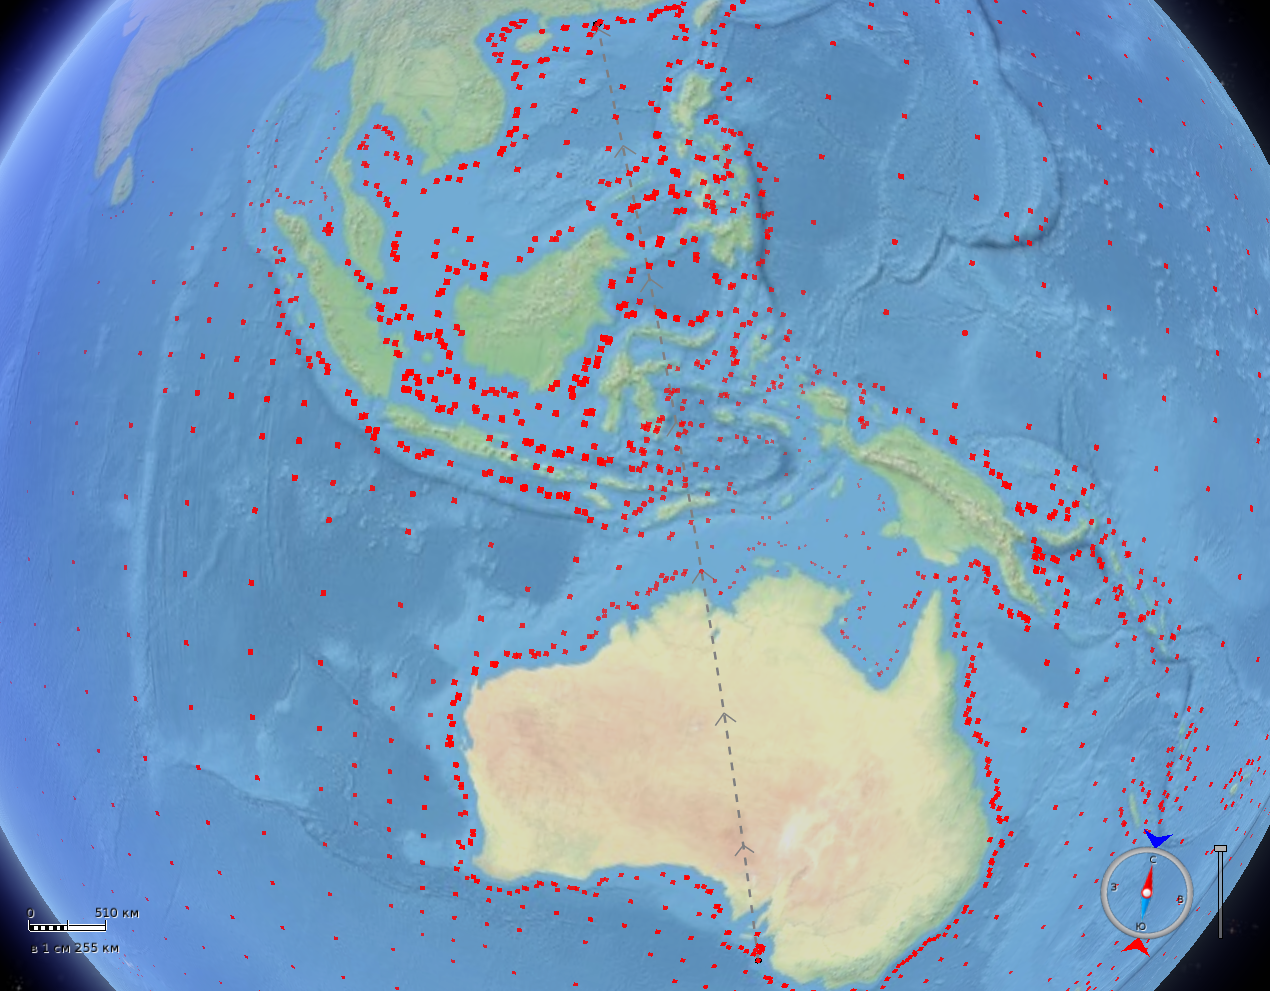
\includegraphics[clip=true, trim = 280pt 0 20pt 0, width=\textwidth]{potentials-update/max4}
            \end{figure}
        \end{columns}
        
        \begin{center}
            При обновлении потенциалов следует брать максимум.
        \end{center}
    }
   
    \only<6> {
        \begin{columns}
            \column{.5\textwidth}
            \begin{figure}
                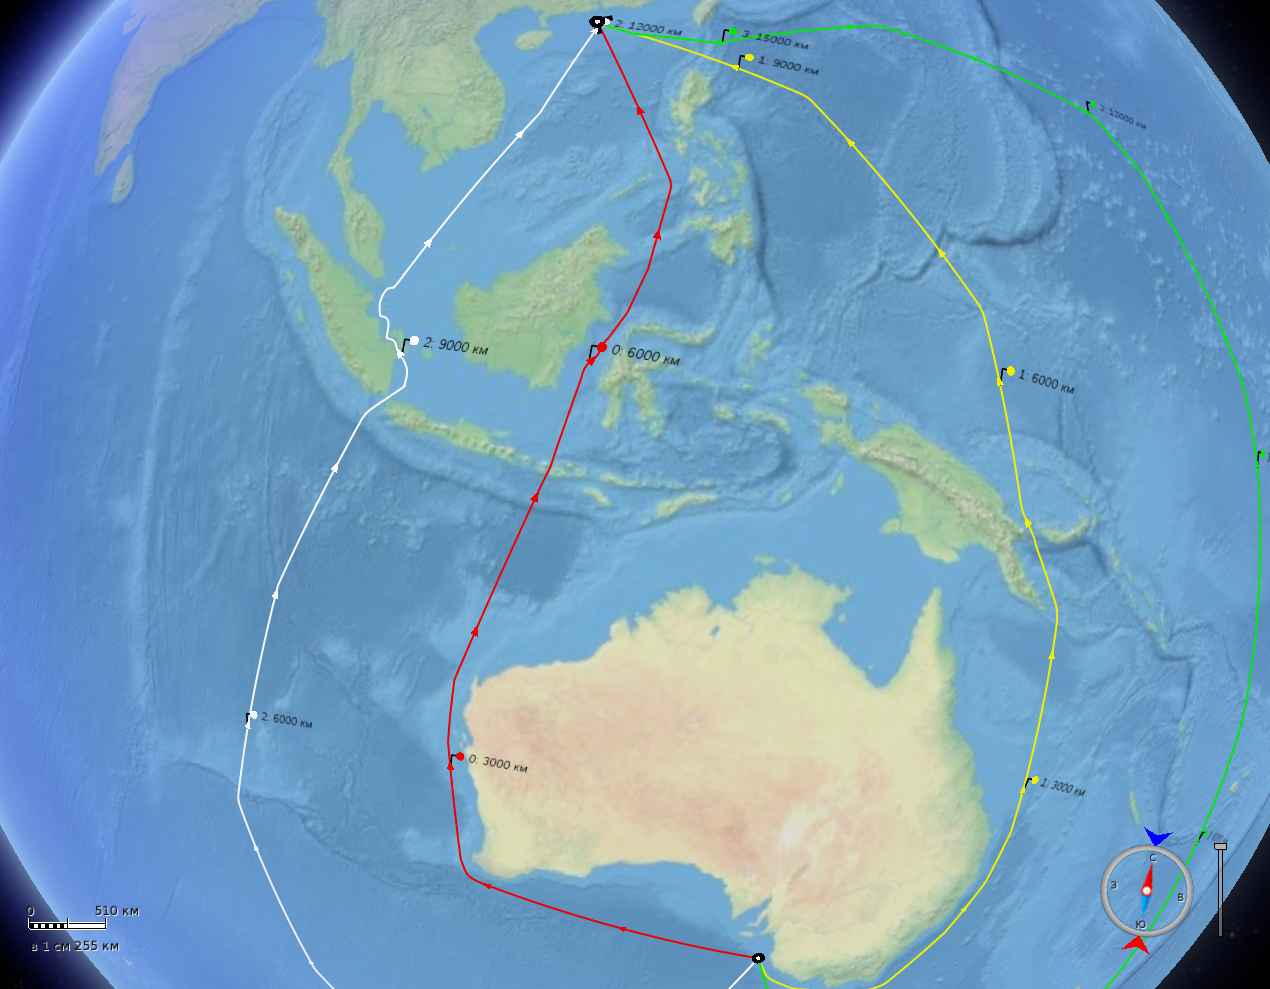
\includegraphics[clip=true, trim = 280pt 0 20pt 0, width=\textwidth]{potentials-update/accum_result}
            \end{figure}

            \column{.5\textwidth}
            \begin{figure}
                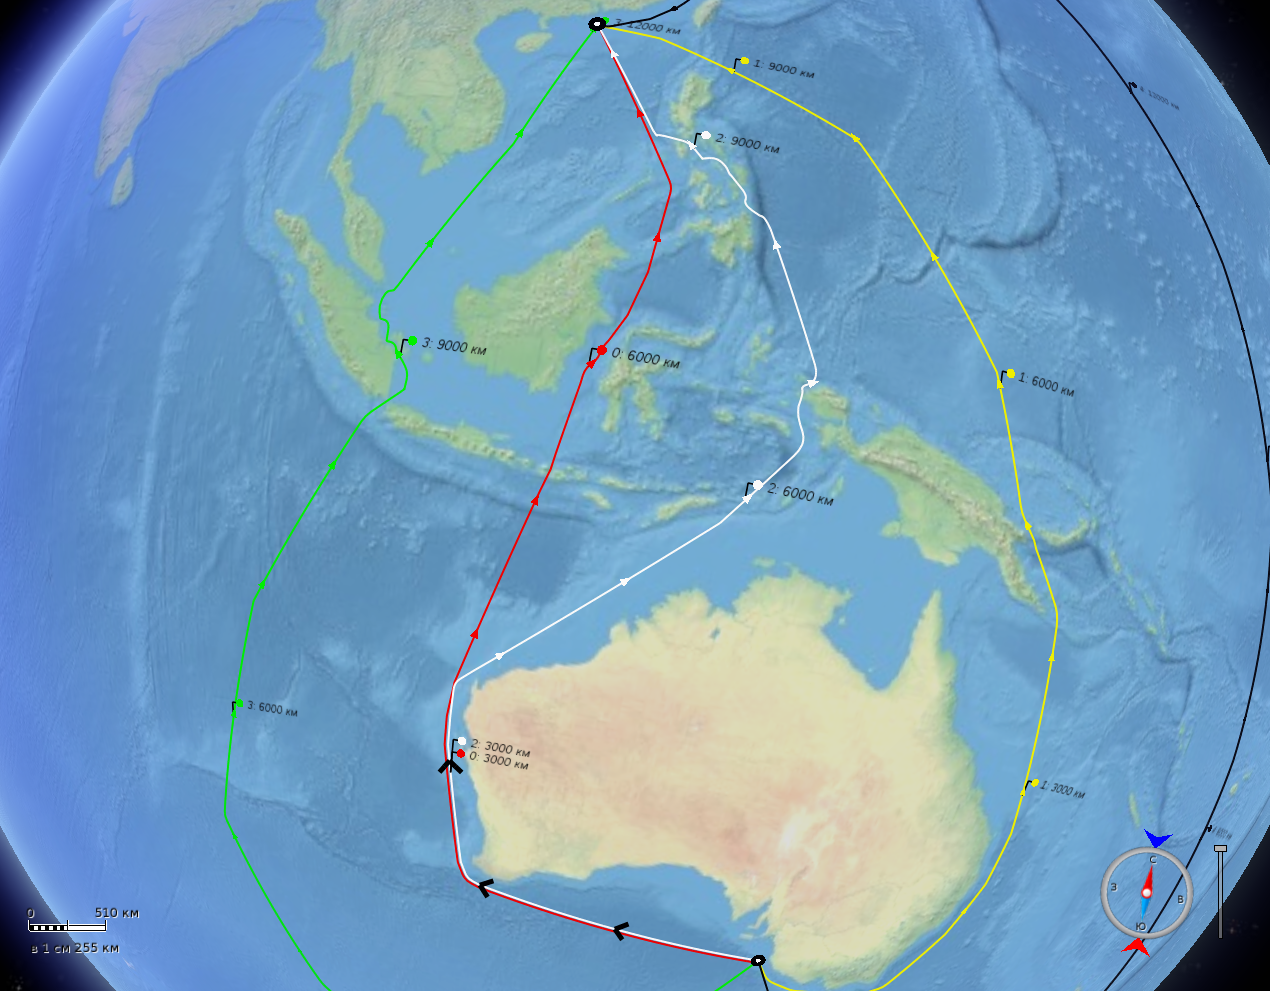
\includegraphics[clip=true, trim = 280pt 0 20pt 0, width=\textwidth]{potentials-update/max_result}
            \end{figure}
        \end{columns}
        
        \begin{center}
            При обновлении потенциалов следует брать максимум.
        \end{center}
    }
   
    \only<7> {
        \begin{figure}
          \begin{columns}
            \column{.5\textwidth}
            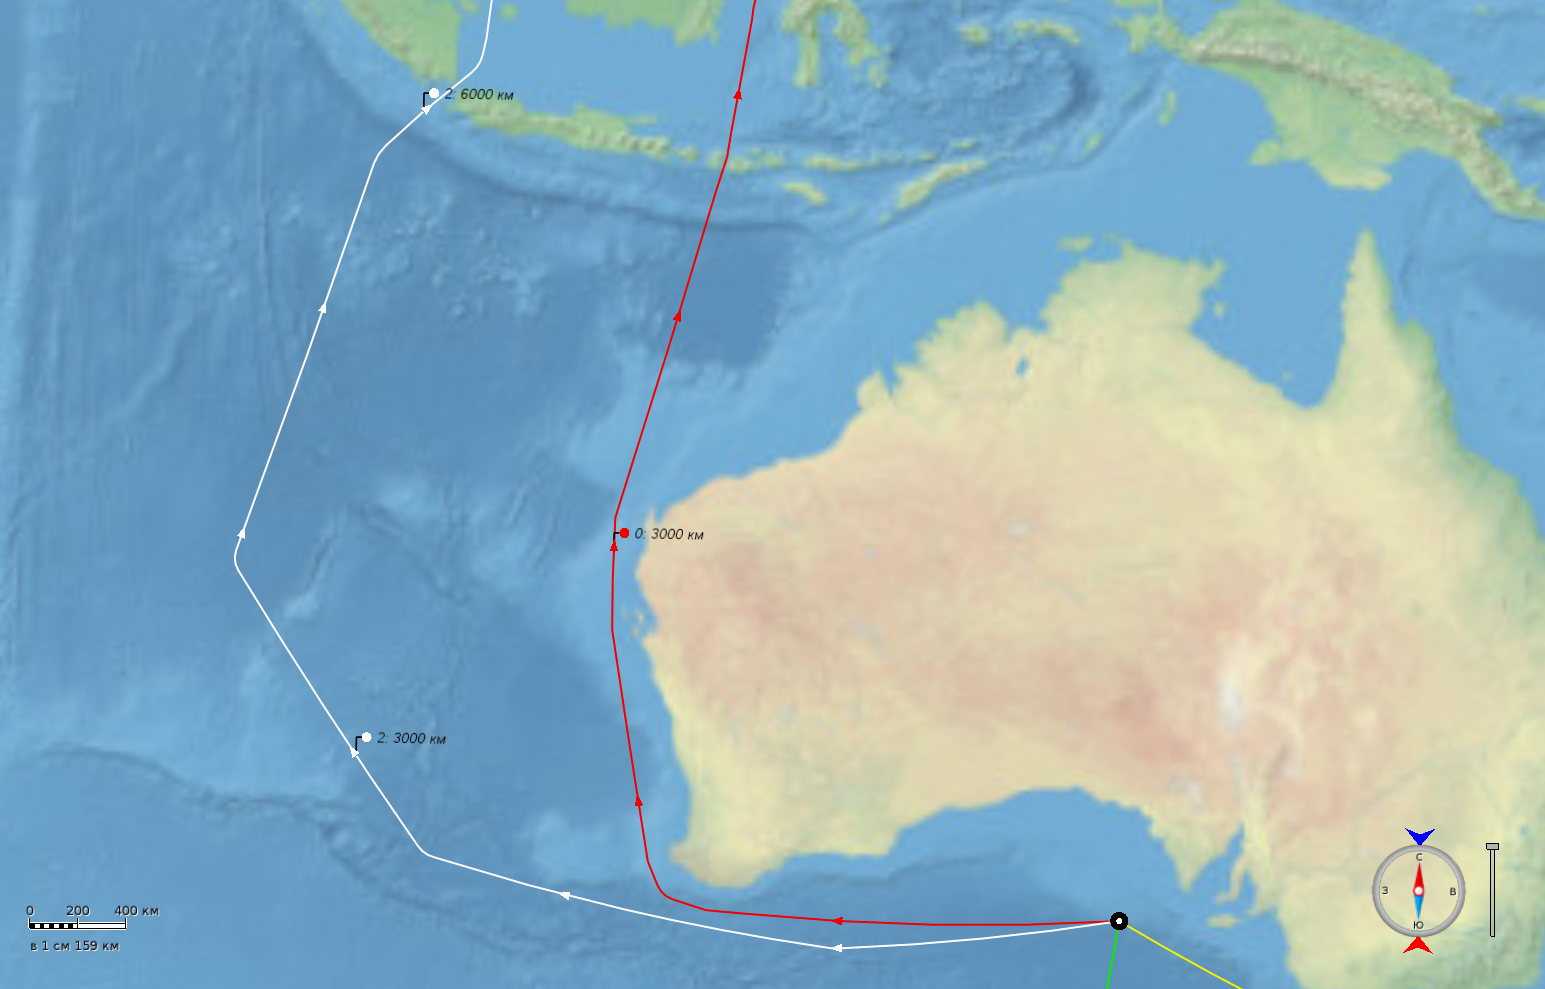
\includegraphics[clip=true, trim = 300pt 20pt 330pt 350pt, width=\textwidth]{weights-on-path-bad}

            \column{.5\textwidth}
            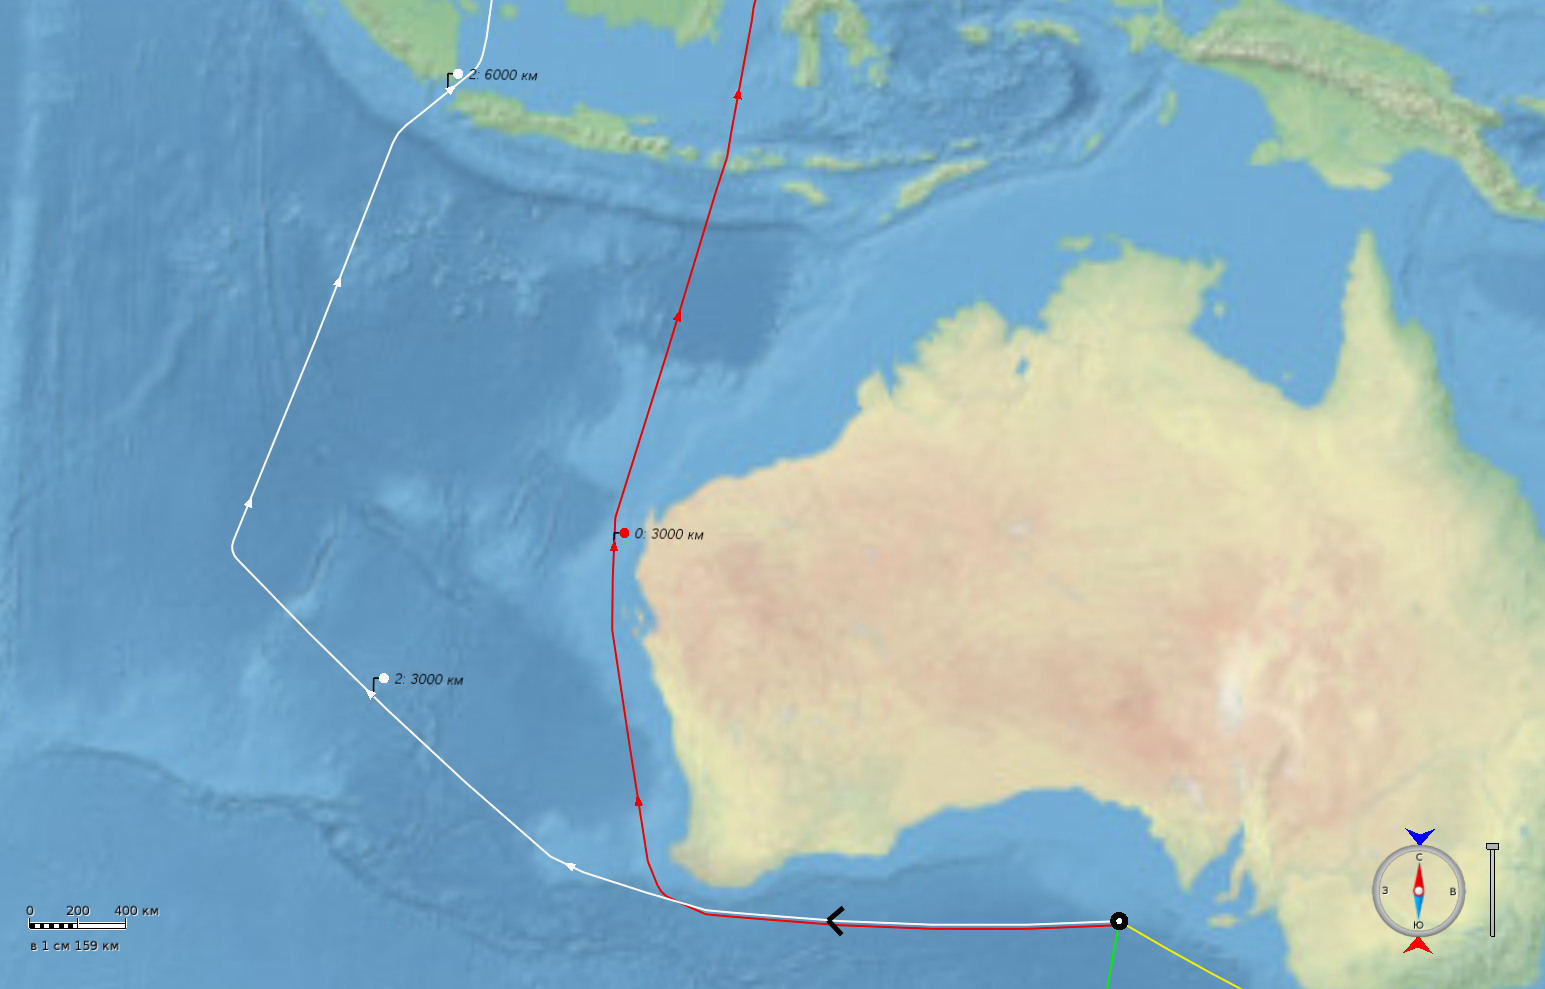
\includegraphics[clip=true, trim = 300pt 20pt 330pt 350pt, width=\textwidth]{weights-on-path-good}
          \end{columns}

            На маршруте потенциалы меньше, чем поблизости
        \end{figure}
    }
\end{frame}
\note {
Остановимся поподробней на обновлении весов.

1. Рассмотрим такую ситуацию, вершины находятся довольно близко,
поэтому их потенциалы примерно равны какому-то C. При этом, если
прибавлять среднее арифметическое, то стоимость верхнего пути
получится на C больше, хотя он лучше. Поэтому будем домножать на
среднее геометрическое. В таком случае вклад потенциалов будет
примерно равен, и будет найден верхний маршрут.

2. Слева показана ситуация, где потенциалы аккумулируются, а справа —
где берётся максимум. Во первом случае почти весь вклад потенциалов
сосредоточен в начале и конце. И в результате эксперимента во втором
случае оказалось найдено на один маршрут больше.

3. Если потенциал монотонно убывает с ростом кратчайшего расстояния от
найденнного маршрута, то на маршруте будут самые большие потенциалы,
поэтому следующий маршрут может отличаться в местах, где он ожидается
таким же. Для получения более естественного результата немного
уменьшим потенциалы вершин маршрута.
}

\begin{frame}{Метрики}
\end{frame}

\begin{frame}{Вычисление метрик}
    \begin{itemize}
        \item Фиктивная вершина
        \item Обход Дейкстры, пока не посещены вершины второго пути 
        \item Заканчиваем, если достигли необходимого значения
        \item Поиск ближайшей вершины (вторая метрика) — перебором
        \item На практике затраты как на первую, так и на вторую
          метрику небольшие
    \end{itemize}
\end{frame}

\section{Результаты}

\begin{frame}{Результаты}
    \only<1> {
        \begin{itemize}
            \item Разработан и реализован алгоритм построения семейств оптимальных маршрутов 
            \item Проведено сравнение с существующими подходами 
            \item Поиск выполняется примерно за полсекунды 
            \item Используется в 3D-клиенте ЗАО «Кронштадт Технологии»
        \end{itemize}
    }
    \only<2> {
        \begin{figure}
            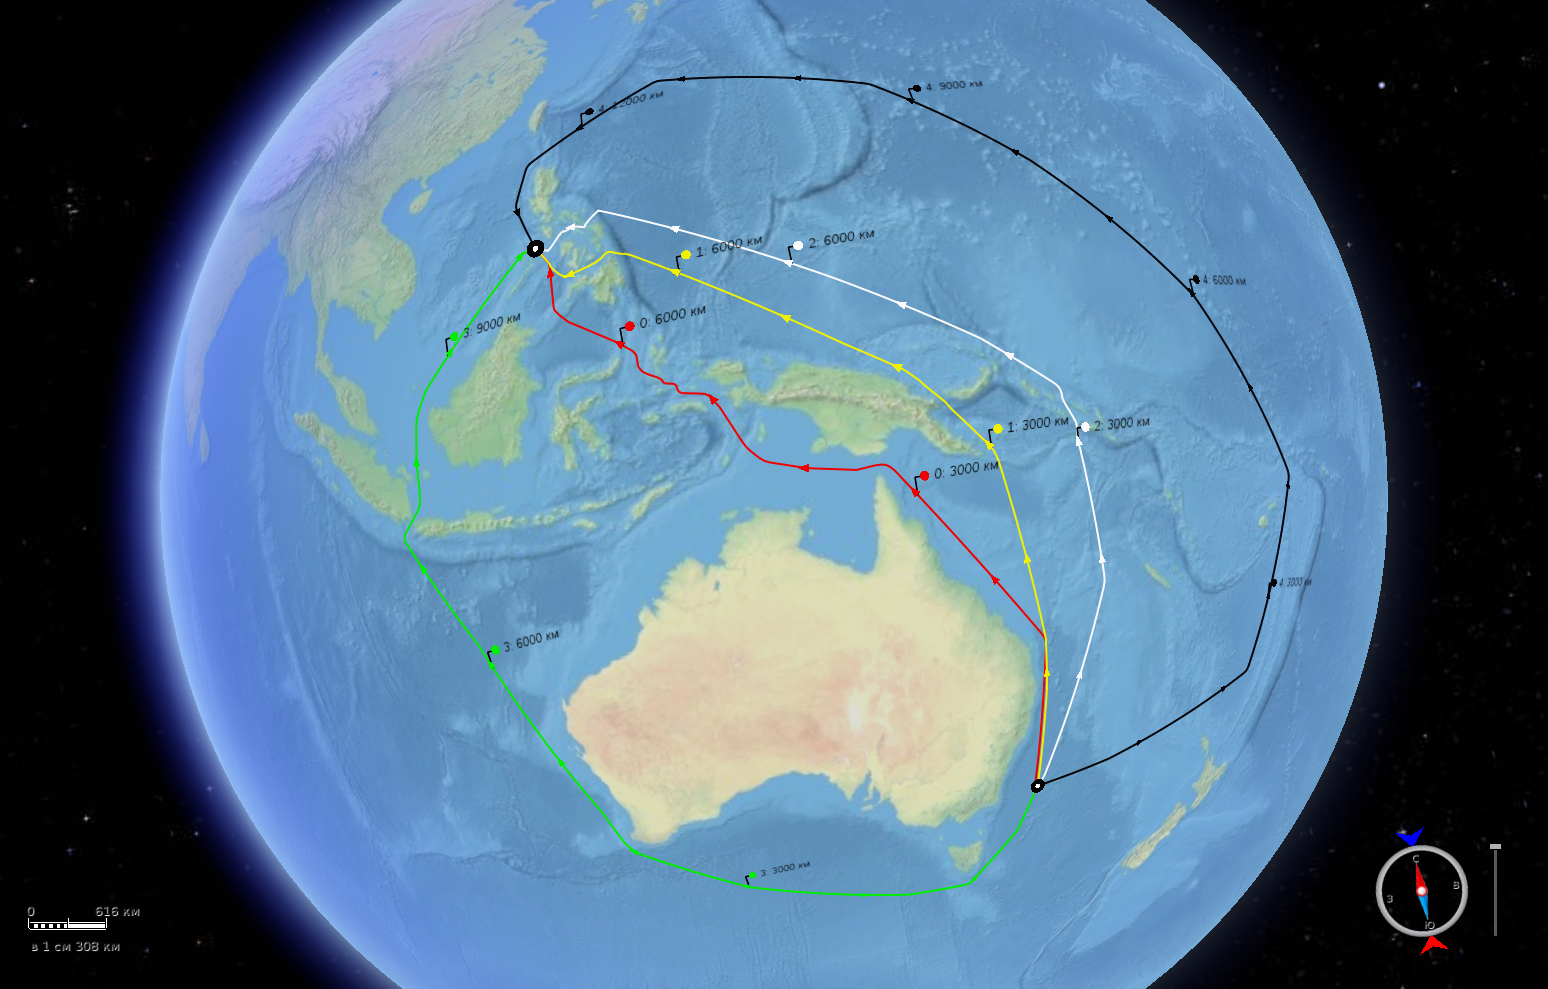
\includegraphics[width=\textwidth]{results/1}
        \end{figure}
    }

    \only<3> {
        \begin{figure}
            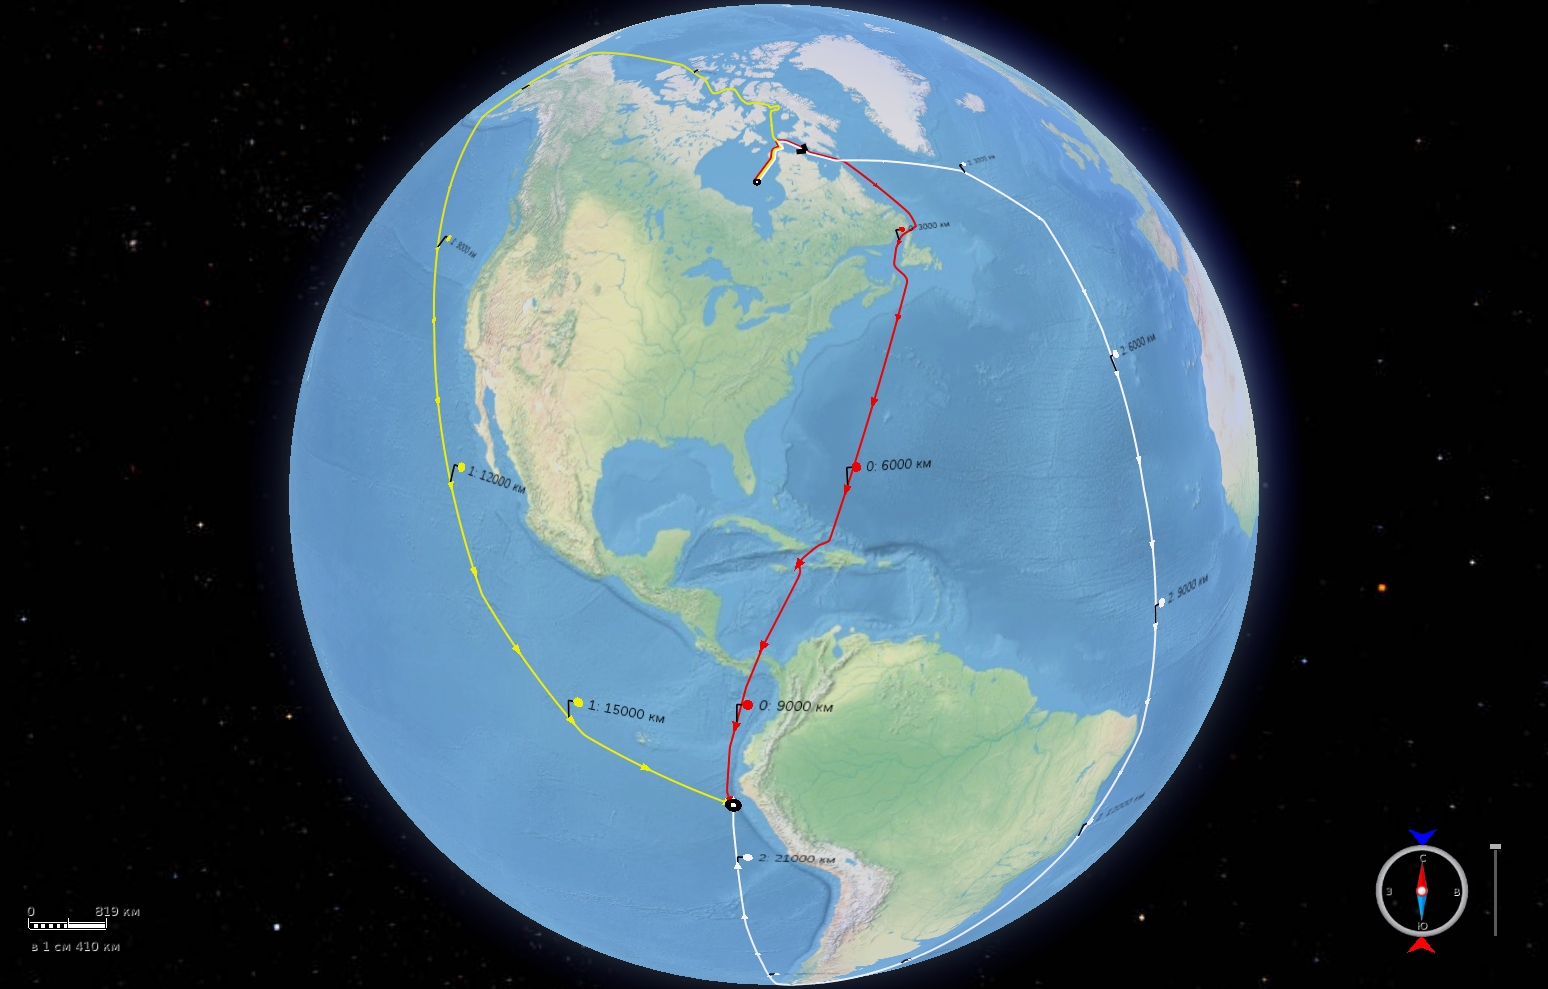
\includegraphics[width=\textwidth]{results/2}
        \end{figure}
    }

    \only<4> {
        \begin{figure}
            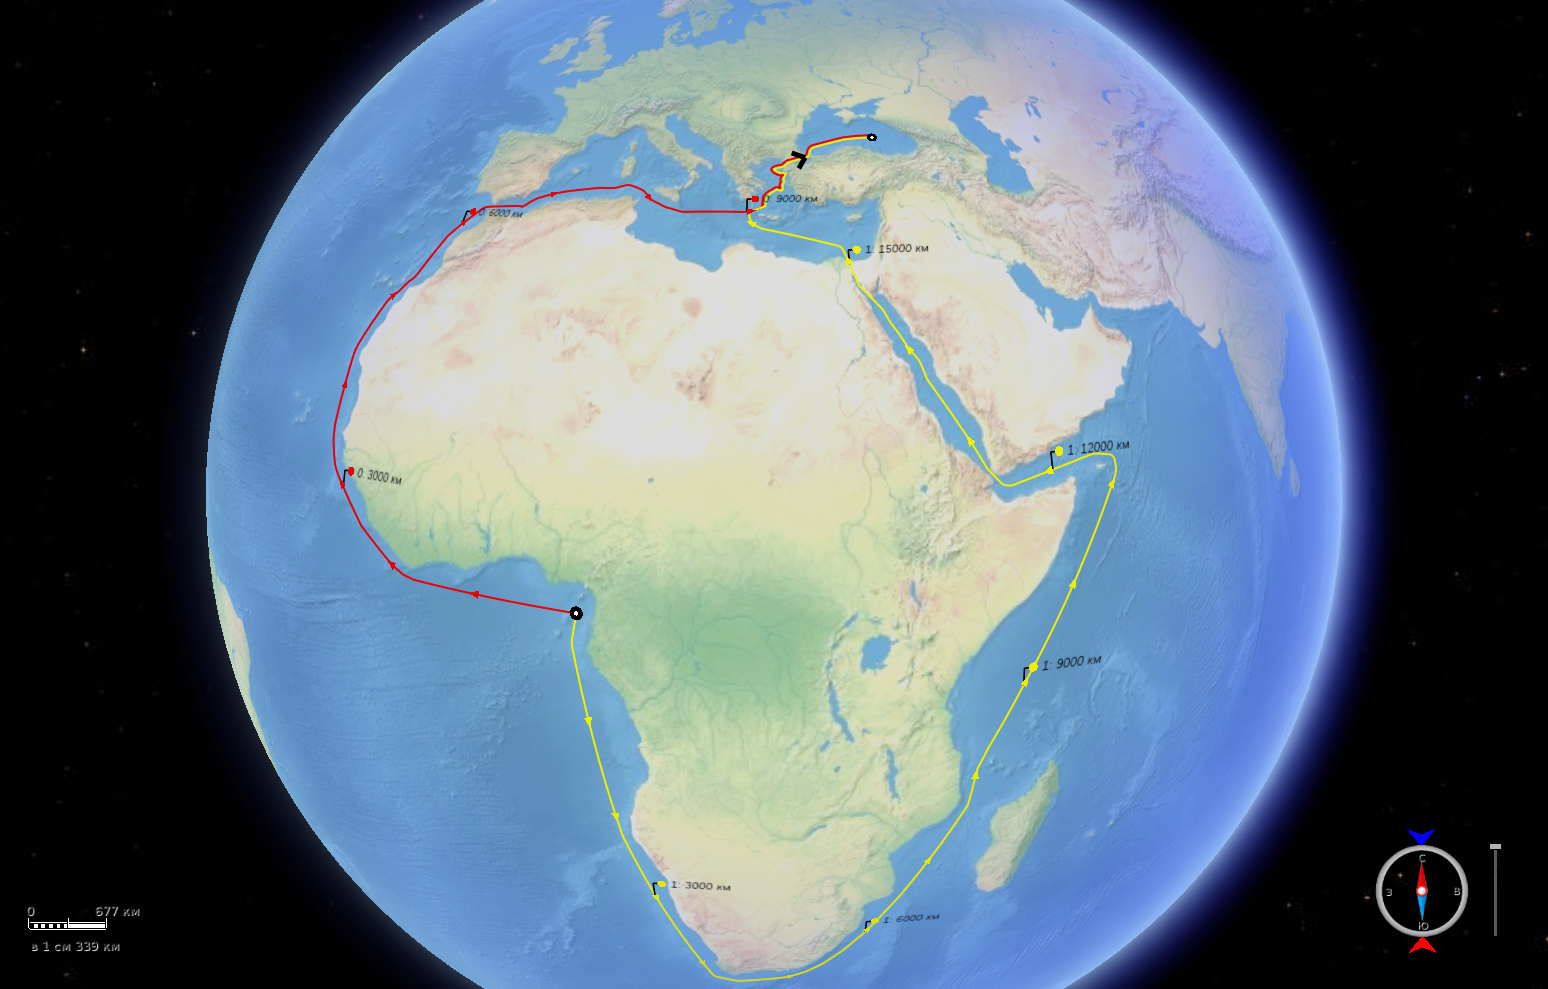
\includegraphics[width=\textwidth]{results/3}
        \end{figure}
    }

\end{frame}
\note {
TODO: экспертное заключение
}

\begin{frame}{Спасибо за внимание!}
    \begin{center}
        \Huge
        {\color{blue} Вопросы?}
    \end{center}
\end{frame}
\note{До свидания!}

\end{document}

